




%---------------------------------------------------------------------

\newpage

%\section[Co-evolution at the meso scale][Co-évolution à l'échelle mesoscopique]{Co-evolution of forms: interactions and morphogenesis at the meso scale}{Co-evolution des formes : interactions et morphogenèse à l'échelle mesoscopique}

\section{Co-evolution at the mesoscopic scale}{Co-évolution à l'échelle mesoscopique}


\label{sec:mesocoevolmodel}

%---------------------------------------------------------------------


\bpar{
Urban settlements and transportation networks have been shown to be co-evolving, in the different thematic, empirical  and modeling studies of territorial systems developed up to here. As we saw, modeling approaches of such dynamical interactions between networks and territories are poorly developed. We propose in this section to realize a first entry at an intermediate scale, focusing on morphological and functional properties of the territorial system in a stylized way. We introduce a stochastic dynamical model of urban morphogenesis which couples the evolution of population density within grid cells with a growing road network.
}{
Les établissements urbains et les réseaux de transport ont été montrés comme co-évolutifs, dans les différentes approches thématiques, empiriques, et de modélisation des systèmes territoriaux développées jusqu'ici. Comme on l'a vu, les approches modélisant ces interactions dynamiques entre réseaux et territoires sont peu développées. Nous proposons dans cette section de réaliser une première entrée à une échelle intermédiaire, en s'intéressant aux propriétés morphologiques et fonctionnelles des systèmes territoriaux de manière stylisée. Nous introduisons un modèle dynamique et stochastique de morphogenèse urbaine qui couple l'évolution de la densité de population dans les cellules d'une grille avec l'évolution d'un réseau routier.
}


%%%%%%%%%%%%%%%%%%
\subsection{Model description}{Description du modèle}


\subsubsection{General structure}{Structure générale}


\bpar{
The general principles of the model are the following. With an overall fixed growth rate, new population aggregate preferentially to a local potential, for which parameters control the dependance to various explicative variables. These are in particular local density, distance to the network, centrality measures within the network and generalized accessibility. \cite{doi:10.1080/13658816.2014.893347} shows in the case of Stockholm the very strong correlation between centrality measures in the network and the type of land-use, what confirms the inportance to consider centralities as explicative variables for the model at this scale. We generalize thus the morphogenesis model studied in~\ref{sec:densitygeneration}, with aggregation mechanisms similar to the ones used by~\cite{raimbault2014hybrid}. A continuous diffusion of population completes the aggregation to translate repulsion processes generally due to congestion. Because of the different time scales of evolution for the urban environment and for networks, the network grows at fixed time steps, following the submodel developed in~\ref{sec:networkgrowth}: a first fixed rule ensures connectivity of newly populated patches to the existing network. The different network generation heuristics are then included in the model. We expect the different heuristics to be complementary since for example the gravity model would be more typical of planned top-down network evolution, whereas the biological model will translate bottom-up processes of network growth. The Fig.~\ref{fig:mesocoevolmodel:workflow} summarizes the general structure of the morphogenesis model.
}{
Les principes généraux du modèle sont les suivants. Avec un taux de croissance global fixé, une nouvelle population s'agrège préférentiellement à un potentiel local, dont la dépendance à diverses variables explicatives est contrôlé par des paramètres. Celles-ci sont la densité locale, la distance au réseau, les mesures de centralité dans le réseau et l'accessibilité généralisée. \cite{doi:10.1080/13658816.2014.893347} montre dans le cas de Stockholm la très forte corrélation entre mesures de centralité et le type d'usage du sol, ce qui confirme l'importance de considérer les centralités comme variables explicatives pour le modèle à cette échelle. Nous généralisons ainsi le modèle de morphogenèse étudié dans~\ref{sec:densitygeneration}, avec des mécanismes d'agrégation similaires à ceux utilisés par~\cite{raimbault2014hybrid}. Une diffusion continue de la population complète l'agrégation pour traduire les processus de répulsion généralement dus à la congestion. À cause des différentes échelles de temps impliquées dans l'évolution de l'environnement urbain et des réseaux, le réseau croit à pas de temps fixés, suivant le sous-modèle développé en~\ref{sec:networkgrowth} : une première règle fixe assure la connectivité des cellules nouvellement peuplés au réseau existant. Les différentes heuristiques de génération de réseau sont ensuite incluses dans le modèle. Nous nous attendons à une complémentarité de celles-ci, puisque par exemple le modèle gravitaire sera plus typique d'une évolution de réseau planifiée, tandis que le modèle biologique traduit des processus auto-organisés de croissance de réseau. La Fig.~\ref{fig:mesocoevolmodel:workflow} résume la structure générale du modèle de morphogenèse.
}




%%%%%%%%%%%%%%%
\begin{figure}
	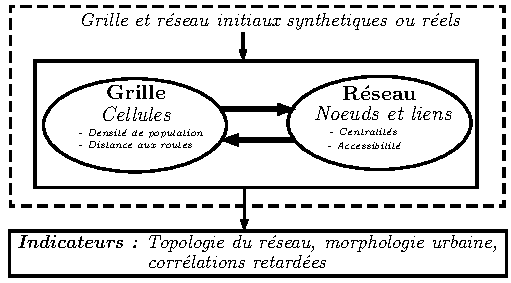
\includegraphics[width=\linewidth]{Figures/MesoCoEvol/mesocoevol_fr.pdf}
	\caption[Morphogenesis at the mesoscopic scale][Morphogenèse mesoscopique]{\textbf{Structure of the co-evolution model at the mesoscopic scale.}\label{fig:mesocoevolmodel:workflow}}{\textbf{Structure du modèle de co-évolution à l'échelle mesoscopique.}\label{fig:mesocoevolmodel:workflow}}
\end{figure}
%%%%%%%%%%%%%%%



\subsubsection{Formalization}{Formalisation}


\bpar{
The model is based on a squared population grid of size $N$, which cells are defined by populations $(P_i)$. A road network is included in a way similar as in~\ref{sec:networkgrowth}. We assume at the initial state a given population distribution and a network.
}{
Le modèle est basé sur une grille carrée de population de côté $N$, dont les cellules sont définies par les populations $(P_i)$. Un réseau routier s'y superpose de la même manière qu'en~\ref{sec:networkgrowth}. Nous supposons une distribution de population à l'instant initial ainsi qu'un réseau.
}


\bpar{
The evolution of densities is based on a utility function, influenced by local characteristics of the urban form and function, that we call \emph{explicative variables}. Let $x_k(i)$ a local explicative variable for cell $i$, which will be among the following variables:
\begin{itemize}
	\item population $P_i$;
	\item proximity to roads\footnote{Taken as $\exp (-d / d_n)$ where $d$ is the distance by projection on the closest road, and $d_n=10$ is fixed.};
	\item betweenness centrality
	\item closeness centrality;
	\item accessibility.
\end{itemize}
For the last three, they are defined as previously for network nodes, and then associated to cells by taking the value of the closest node, weighted by a decreasing function of the distance to it\footnote{I.e. of the form $x_k = x^{(n)}_k (\argmin_j d(i,j)) \cdot \exp \left( -  \min_j d(i,j) / d_0 \right)$, with $x^{(n)}_k$ the corresponding variable for nodes, the index $j$ being taken on all nodes, and the decay parameter $d_0$ is in our case fixed at $d_0=1$ to keep the property that network variables are essentially significant at close distances from the network.}. We consider then normalized explicative variables defined by $\tilde{x}_k(i) = x_k(i) - \min_j x_k(j) / (\max_j x_k(j) - \min_j x_k(j))$.
}{
L'évolution des densités se base sur une fonction d'utilité, influencée par des caractéristiques locales de la forme et de la fonction urbaine, que l'on appelle \emph{variables explicatives}. Soit $x_k(i)$ une variable explicative locale pour la cellule $i$, qui sera parmi les variables suivantes : 
\begin{itemize}
	\item population $P_i$ ;
	\item proximité aux routes\footnote{Prise sous la forme $\exp (-d / d_n)$ avec $d$ distance par projection sur la route la plus proche, et $d_n =10$ fixé.} ;
	\item centralité de chemin ;
	\item centralité de proximité ;
	\item accessibilité.
\end{itemize}
Pour les trois dernières, celles-ci sont définies comme précédemment pour les noeuds du réseau, puis associées aux cellules en prenant la valeur du noeud le plus proche, pondérée par une fonction décroissante en fonction de la distance à celui-ci\footnote{C'est-à-dire de la forme $x_k = x^{(n)}_k (\argmin_j d(i,j)) \cdot \exp \left( -  \min_j d(i,j) / d_0 \right)$, avec $x^{(n)}_k$ variable correspondante pour les noeuds, l'indice $j$ étant pris sur l'ensemble des noeuds, et le paramètre de décroissance $d_0$ étant dans notre cas fixé à $d_0 = 1$ pour garder la caractéristique que les variables de réseau sont essentiellement significatives à des distances proches de celui-ci.}. Nous considérons alors les variables explicatives normalisées définies par $\tilde{x}_k(i) = x_k(i) - \min_j x_k(j) / (\max_j x_k(j) - \min_j x_k(j))$. 
}



\bpar{
The utility of a cell is then given by a linear aggregation\footnote{An alternative could be for example a Cobb-Douglas function, which is equivalent to a linear aggregation on the logarithms of variables.}
\begin{equation}
U_i = \sum_k w_k \cdot \tilde{x}_k(i)
\end{equation}
where $\tilde{x}_k$ are the normalized local explicative variables, and $w_k$ are weight parameters, which allow to weight between the different influences.
}{
L'utilité d'une cellule est alors donnée par une agrégation linéaire\footnote{Une alternative étant par exemple une fonction de Cobb-Douglas, qui revient à une agrégation linéaire sur les logarithmes des variables.}
\begin{equation}
U_i = \sum_k w_k \cdot \tilde{x}_k(i)
\end{equation}
où les $\tilde{x}_k$ sont les variables explicatives locales normalisées, et $w_k$ des paramètres de poids, qui permettent de pondérer les différentes influences.
}



\bpar{
A time step of model evolution includes then the following stages.
\begin{enumerate}
	\item Evolution of the population following rules similar to the morphogenesis model developed in~\ref{sec:densitygeneration}. Given an exogenous growth rate $N_G$, individuals are added independently following an aggregation done with a probability $U_i^\alpha/\sum_k U_k^\alpha$, followed by a diffusion of strength $\beta$ to neighbor cells, done $n_d$ times.
	\item Network growth following the rules described in~\ref{sec:networkgrowth}, knowing that this takes place is the time step is a multiple of a parameter $t_N$, which allows to integrate a differential between temporal scales for population growth and for network growth.
\end{enumerate}
}{
Un pas de temps d'évolution du modèle comporte alors les étapes suivantes.
\begin{enumerate}
	\item Évolution de la population selon des règles similaires au modèle de morphogenèse développé en~\ref{sec:densitygeneration}. Étant donné un taux de croissance exogène $N_G$, les individus sont ajoutés de manière indépendante suivant une agrégation faite selon la probabilité $U_i^\alpha/\sum_k U_k^\alpha$, suivie d'une diffusion aux voisins de force $\beta$, effectuée $n_d$ fois.
	\item Croissance du réseau selon les règles décrites en~\ref{sec:networkgrowth}, sachant que celle-ci a lieu si le pas de temps est un multiple d'un paramètre $t_N$, qui permet d'intégrer un différentiel d'échelles temporelles entre la croissance de la population et celle du réseau.
\end{enumerate}
}


\bpar{
The aggregation following a power of the utility yields a flexibility in the underlying optimization problem, since as \cite{josselin2013revisiting} recall, the use of different norms in spatial optimal location problems corresponds to different logics of optimization.
}{
L'agrégation selon une puissance de l'utilité permet une flexibilité dans le problème d'optimisation sous-jacent, puisque comme le rappellent \cite{josselin2013revisiting} l'utilisation de différentes normes dans les problèmes de localisation spatiale optimale correspond à des logiques d'optimisation différentes.
}


\bpar{
The parameters of the model that we will make vary are then:
\begin{itemize}
	\item aggregation-diffusion parameters $\alpha,\beta,N_g,n_d$, summarized in Table~\ref{tab:density:parameters};
	\item the four weight parameters $w_k$ for the explicative variables, which vary in $[0;1]$;
	\item network growth parameters for the different heuristics, summarized in Table~\ref{tab:networkgrowth:parameters}.
\end{itemize}
}{
Les paramètres du modèle que nous ferons varier sont donc :
\begin{itemize}
	\item les paramètres d'agrégation-diffusion $\alpha,\beta,N_g,n_d$, résumés en Table~\ref{tab:density:parameters} ;
	\item les paramètres de poids des variables explicatives $w_k$, au nombre de 4, compris dans $[0;1]$ ;
	\item les paramètres de croissance de réseau des différentes heuristiques, résumés en Table~\ref{tab:networkgrowth:parameters}.
\end{itemize}
}


\bpar{
Output model indicators are the urban morphology indicators, topological network indicators, and lagged correlations between the different explicative variables.
}{
Les indicateurs de sortie du modèle sont les indicateurs de morphologie urbaine, les indicateurs topologiques du réseau, et les corrélations retardées entre les différentes variables explicatives.
}


%%%%%%%%%%%%%%%%%%%
\subsection{Results}{Résultats}

\subsubsection{Implementation}{Implémentation}

\bpar{
The model is implemented in NetLogo, given the heterogeneity of aspects that have to be taken into account, and this language being particularly suitable to couple a grid of cells with a network. Urban morphology indicators are computed thanks to a NetLogo extension specially developed (see Appendix~\ref{app:tools}).
}{
Le modèle est implémenté en NetLogo, vu l'hétérogénéité des aspects à prendre en compte, et ce langage se montrant particulièrement efficace pour coupler une grille de cellules à un réseau. Les indicateurs de morphologie urbaine sont calculés grâce à une extension NetLogo spécifiquement développée (voir Annexe~\ref{app:tools}).
}



\subsubsection{Experience plan}{Plan d'expérience}


\bpar{
We propose to focus on the ability of the model to capture relations between networks and territories, and more particularly the co-evolution. Therefore, we will try to establish if (i) the model is able to reproduce, beyond the form indicators, the static correlation matrices computed in~\ref{sec:staticcorrelations}; and (ii) the model produces a variety of dynamical relations in the sense of causality regimes developed in~\ref{sec:causalityregimes}.
}{
Nous proposons de nous concentrer sur la capacité du modèle à capturer les relations entre réseaux et territoires, et en particulier la co-évolution. Pour cela, nous chercherons si (i) le modèle est capable de reproduire, en plus des indicateurs de forme, les matrices de corrélations statiques calculées en~\ref{sec:staticcorrelations} ; et (ii) le modèle produit une variété de relations dynamiques au sens des régimes de causalité développés en~\ref{sec:causalityregimes}.
}


\bpar{
The model is initialized on fully synthetic configurations, with a grid of size $50$. Configurations are generated through an exponential mixture in a way similar to \cite{anas1998urban}: $N_c = 8$ centers are randomly located, to which a population is attributed following a scaling law $P_i = P_0\cdot (i+1)^{-\alpha_S}$ with $\alpha_S = 0.8$ and $P_0 = 200$. The population of each center is distributed to all cells with an exponential kernel of shape $d(r) = P_{max}\exp\left( - r / r_0\right)$ where the parameter $r_0$ is determined to fix the population at $P_i$, with $P_{max} = 20$ (density at the center)\footnote{We have indeed $P_i = \iint d(r) = \int_{\theta=0}^{2\pi} \int_{r=0}^{\infty} d(r) rdrd\theta = 2 \pi P_{max} \int_r r\cdot \exp\left( - r / r_0\right) = 2 \pi P_{max} r_0^2$, and therefore $r_0 = \sqrt{\frac{P_i}{2\pi P_{max}}}$.}. The initial network skeleton is generated as detailed in~\ref{sec:networkgrowth}.
}{
Le modèle est initialisé sur configurations entièrement synthétiques, avec une taille de grille $50$. Les configurations sont générées par mélange d'exponentielles d'une manière similaire à \cite{anas1998urban} : $N_c = 8$ centres sont localisés de manière aléatoire, et une population leur est attribuée selon une loi d'échelle $P_i = P_0\cdot (i+1)^{-\alpha_S}$ avec $\alpha_S = 0.8$ et $P_0 = 200$. La population de chaque centre est distribuée à l'ensemble des cellules avec un noyau exponentiel de forme $d(r) = P_{max}\exp\left( - r / r_0\right)$ où le paramètre $r_0$ est déterminé pour fixer la population à $P_i$, avec $P_{max} = 20$ (densité au centre)\footnote{On a en effet $P_i = \iint d(r) = \int_{\theta=0}^{2\pi} \int_{r=0}^{\infty} d(r) rdrd\theta = 2 \pi P_{max} \int_r r\cdot \exp\left( - r / r_0\right) = 2 \pi P_{max} r_0^2$, et donc $r_0 = \sqrt{\frac{P_i}{2\pi P_{max}}}$.}. Le squelette de réseau initial est généré comme détaillé en~\ref{sec:networkgrowth}.
}


\bpar{
We explore a Latin Hypercube Sampling of the parameter space, with 10 repetitions for around 7000 parameter points, corresponding to a total of around 70000 model repetitions\footnote{For which simulation results are also available at \url{http://dx.doi.org/10.7910/DVN/OBQ4CS}.}, realized on a computation grid by using OpenMole.
}{
Nous explorons un échantillonnage LHS de l'espace des paramètres, avec 10 répétitions pour environ 7000 points de paramètres, correspondant à un total autour de 70000 répétitions du modèle\footnote{Pour lesquelles les résultats de simulation sont disponibles également à \url{http://dx.doi.org/10.7910/DVN/OBQ4CS}.}, effectuées sur grille de calcul par l'intermédiaire d'OpenMole.
}



\subsubsection{Static and dynamical calibration}{Calibration statique et dynamique}




%%%%%%%%%%%%%%%
\begin{figure}
	%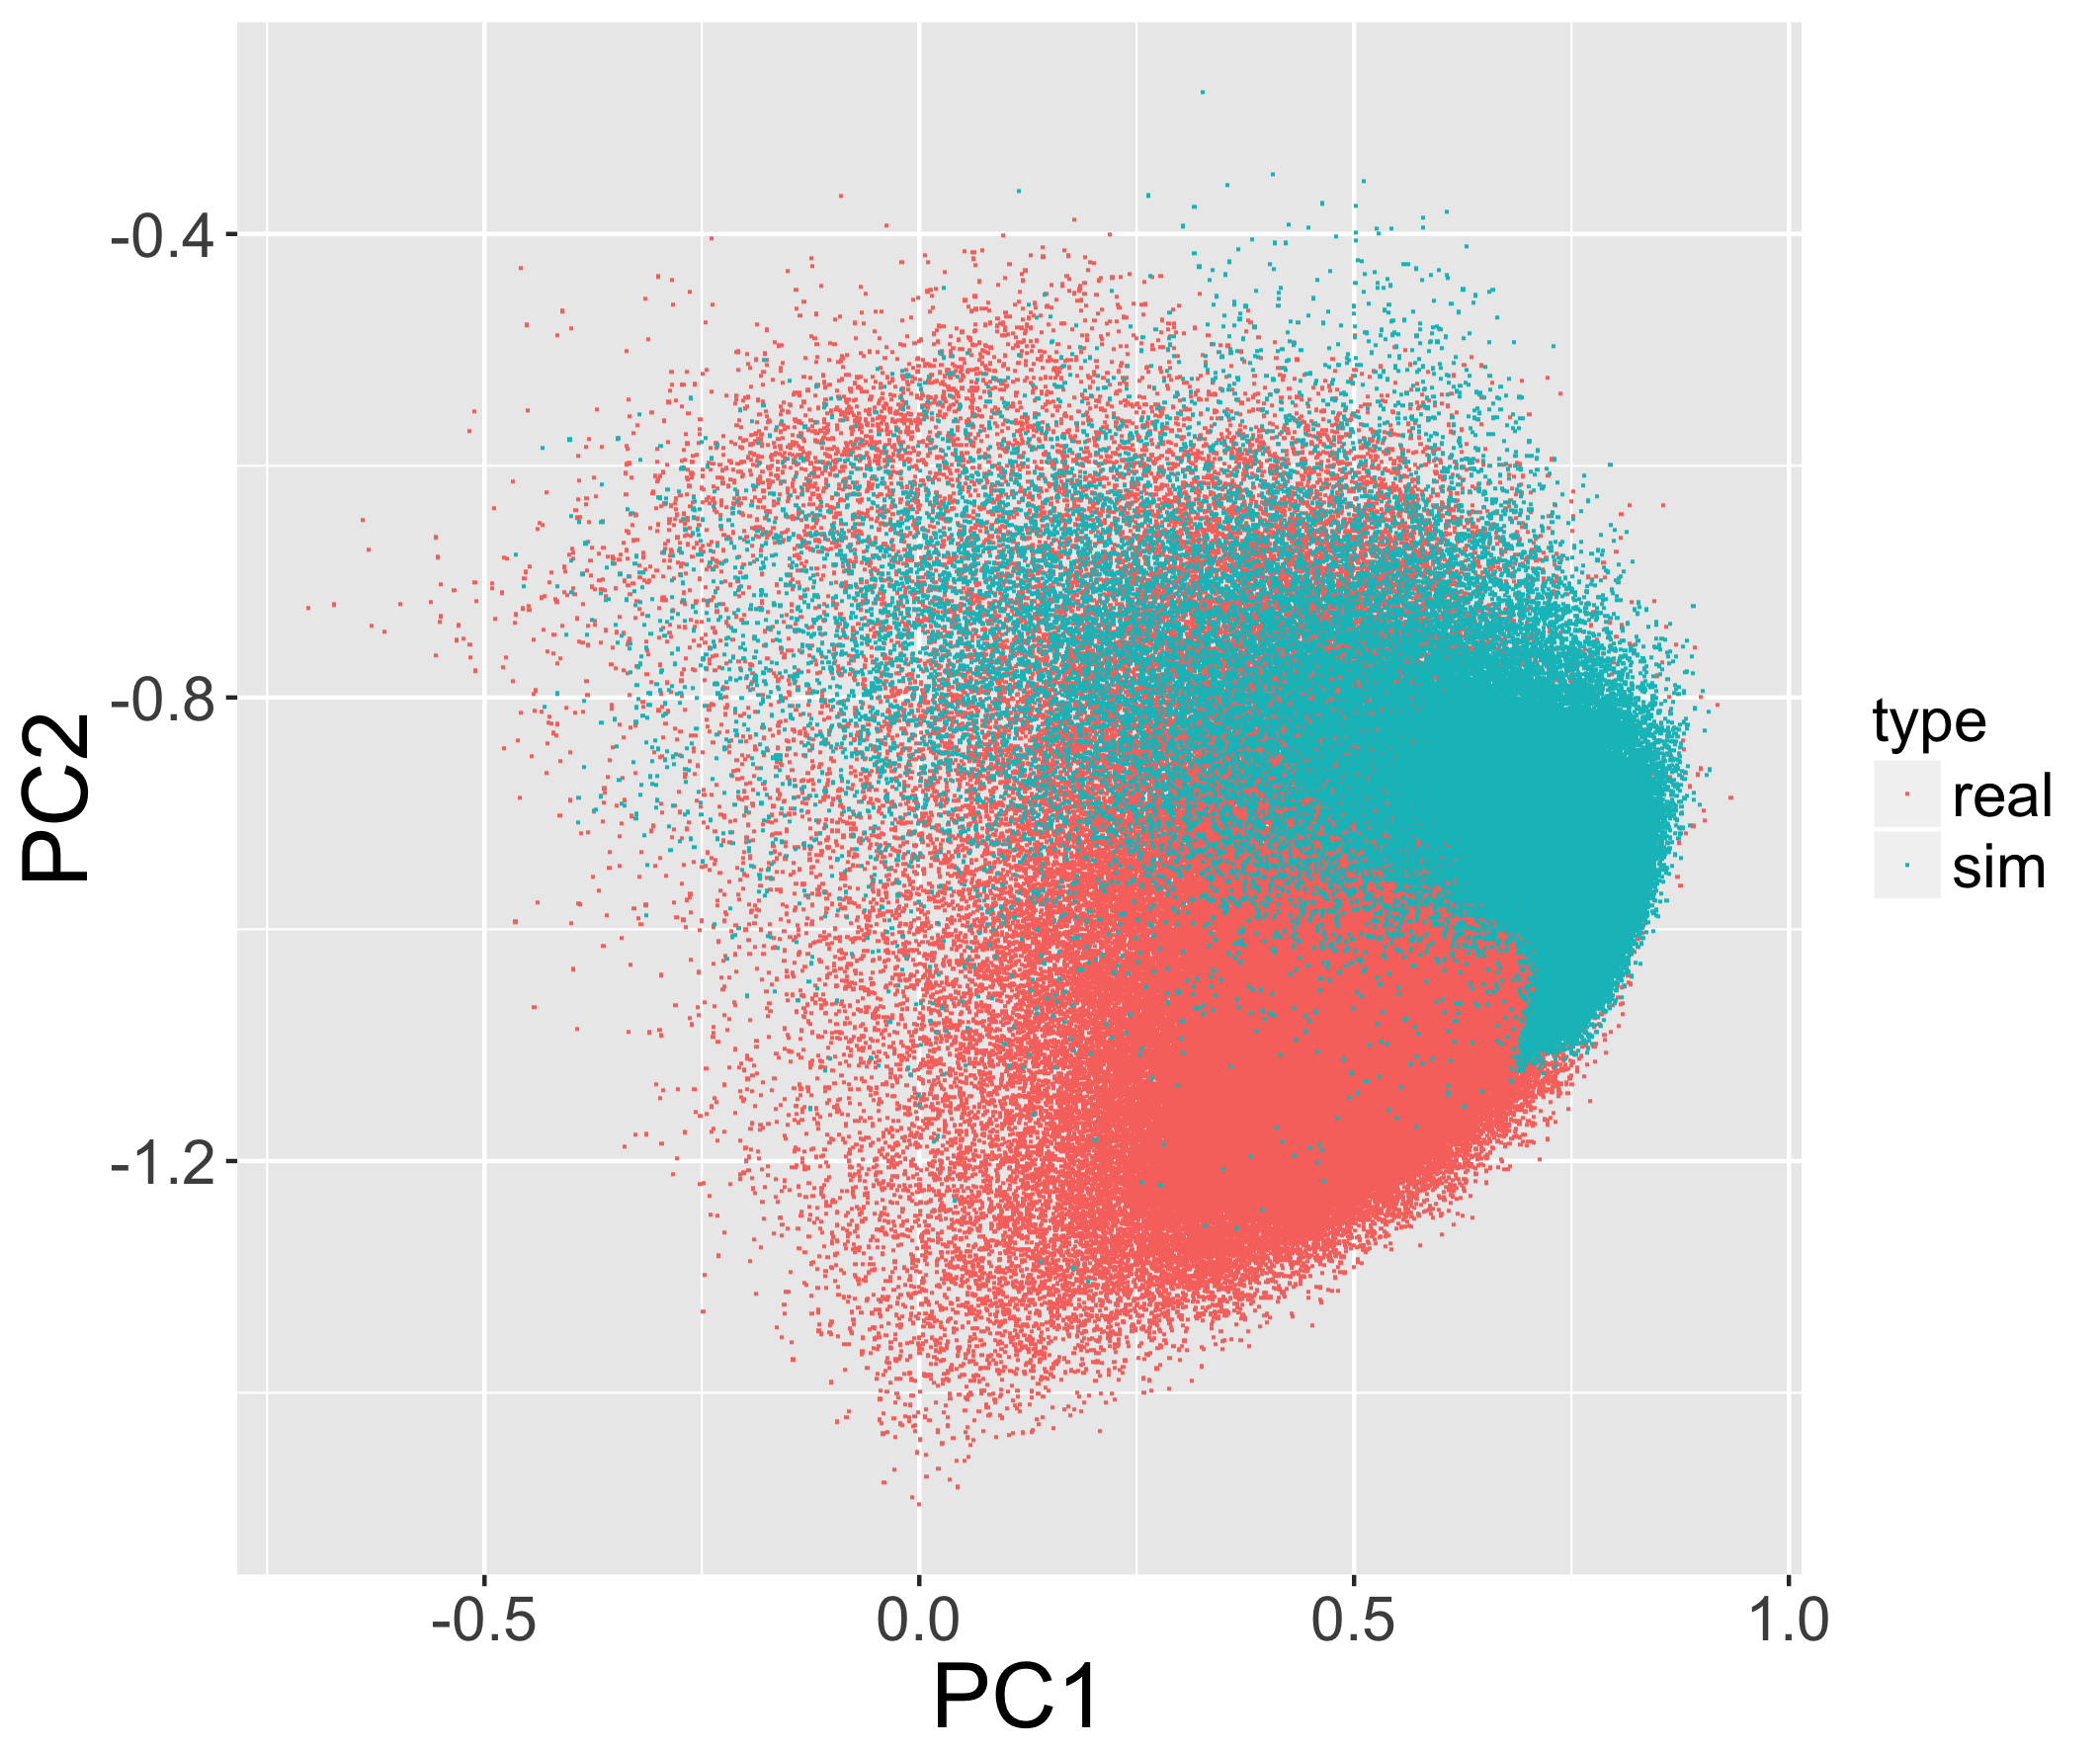
\includegraphics[width=0.48\linewidth]{Figures/MesoCoEvol/pca_allobjs}
	%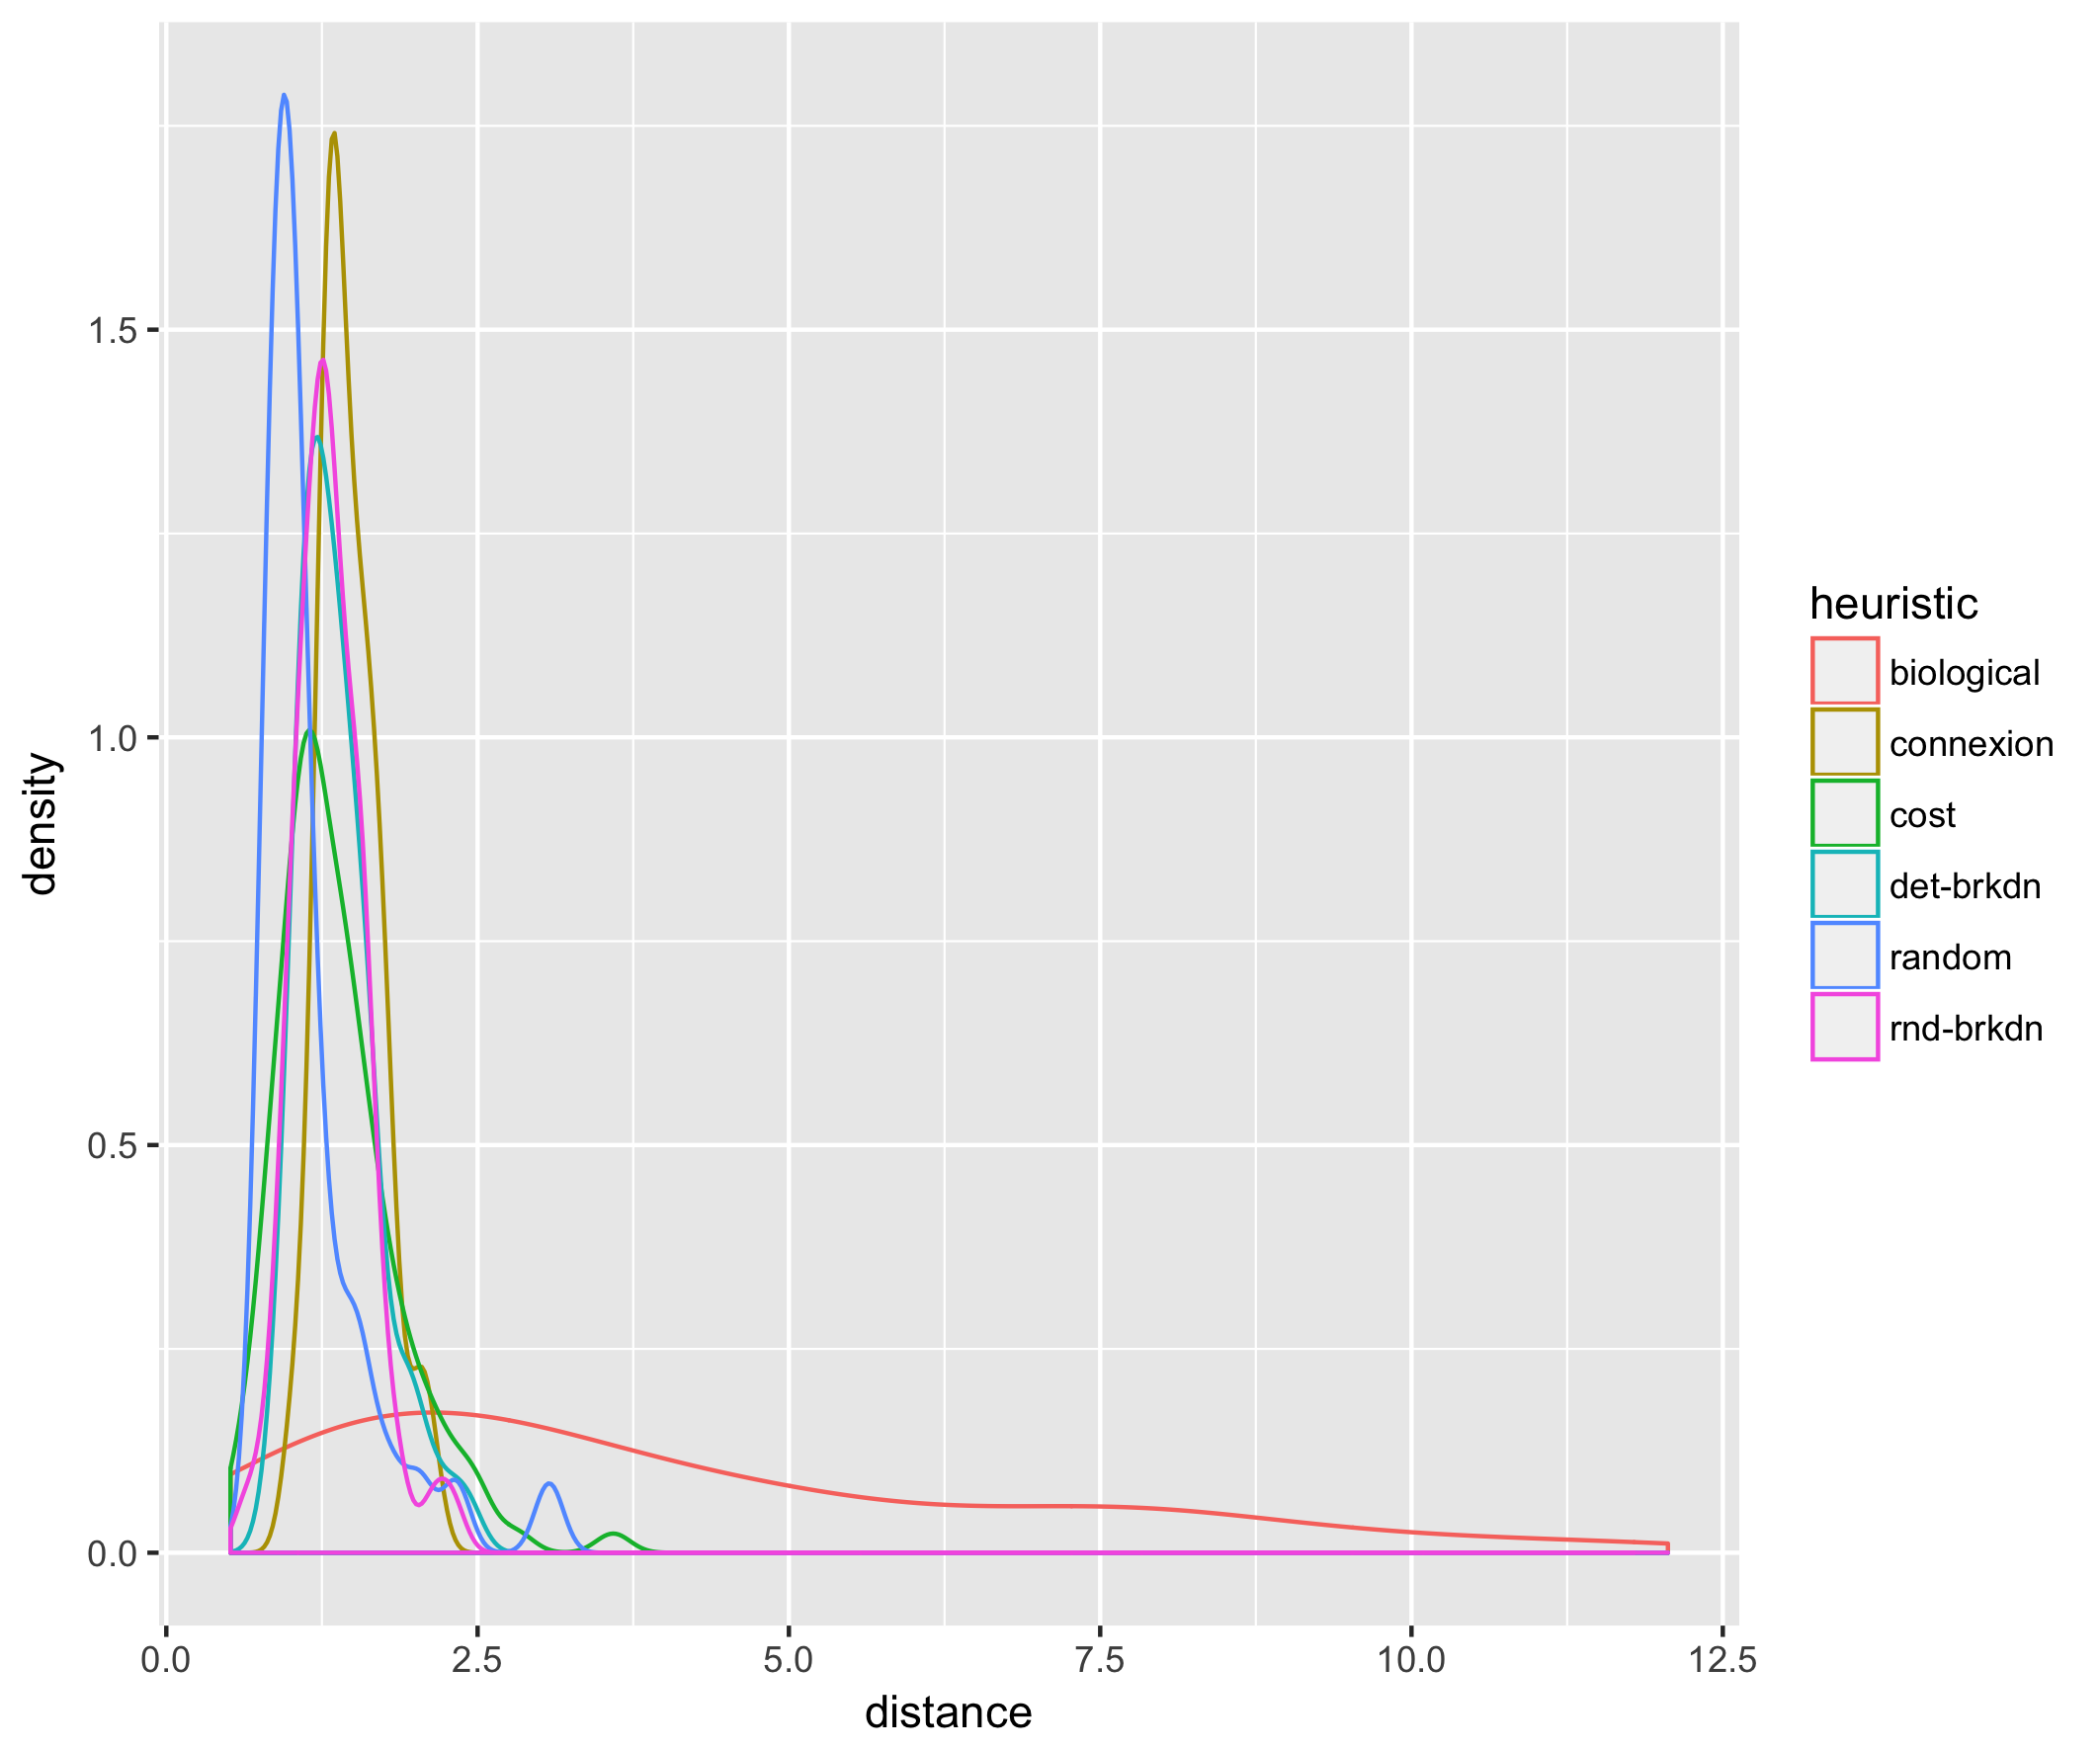
\includegraphics[width=0.48\linewidth]{Figures/MesoCoEvol/corrs-distrib_rhoasize4.png}\\
	%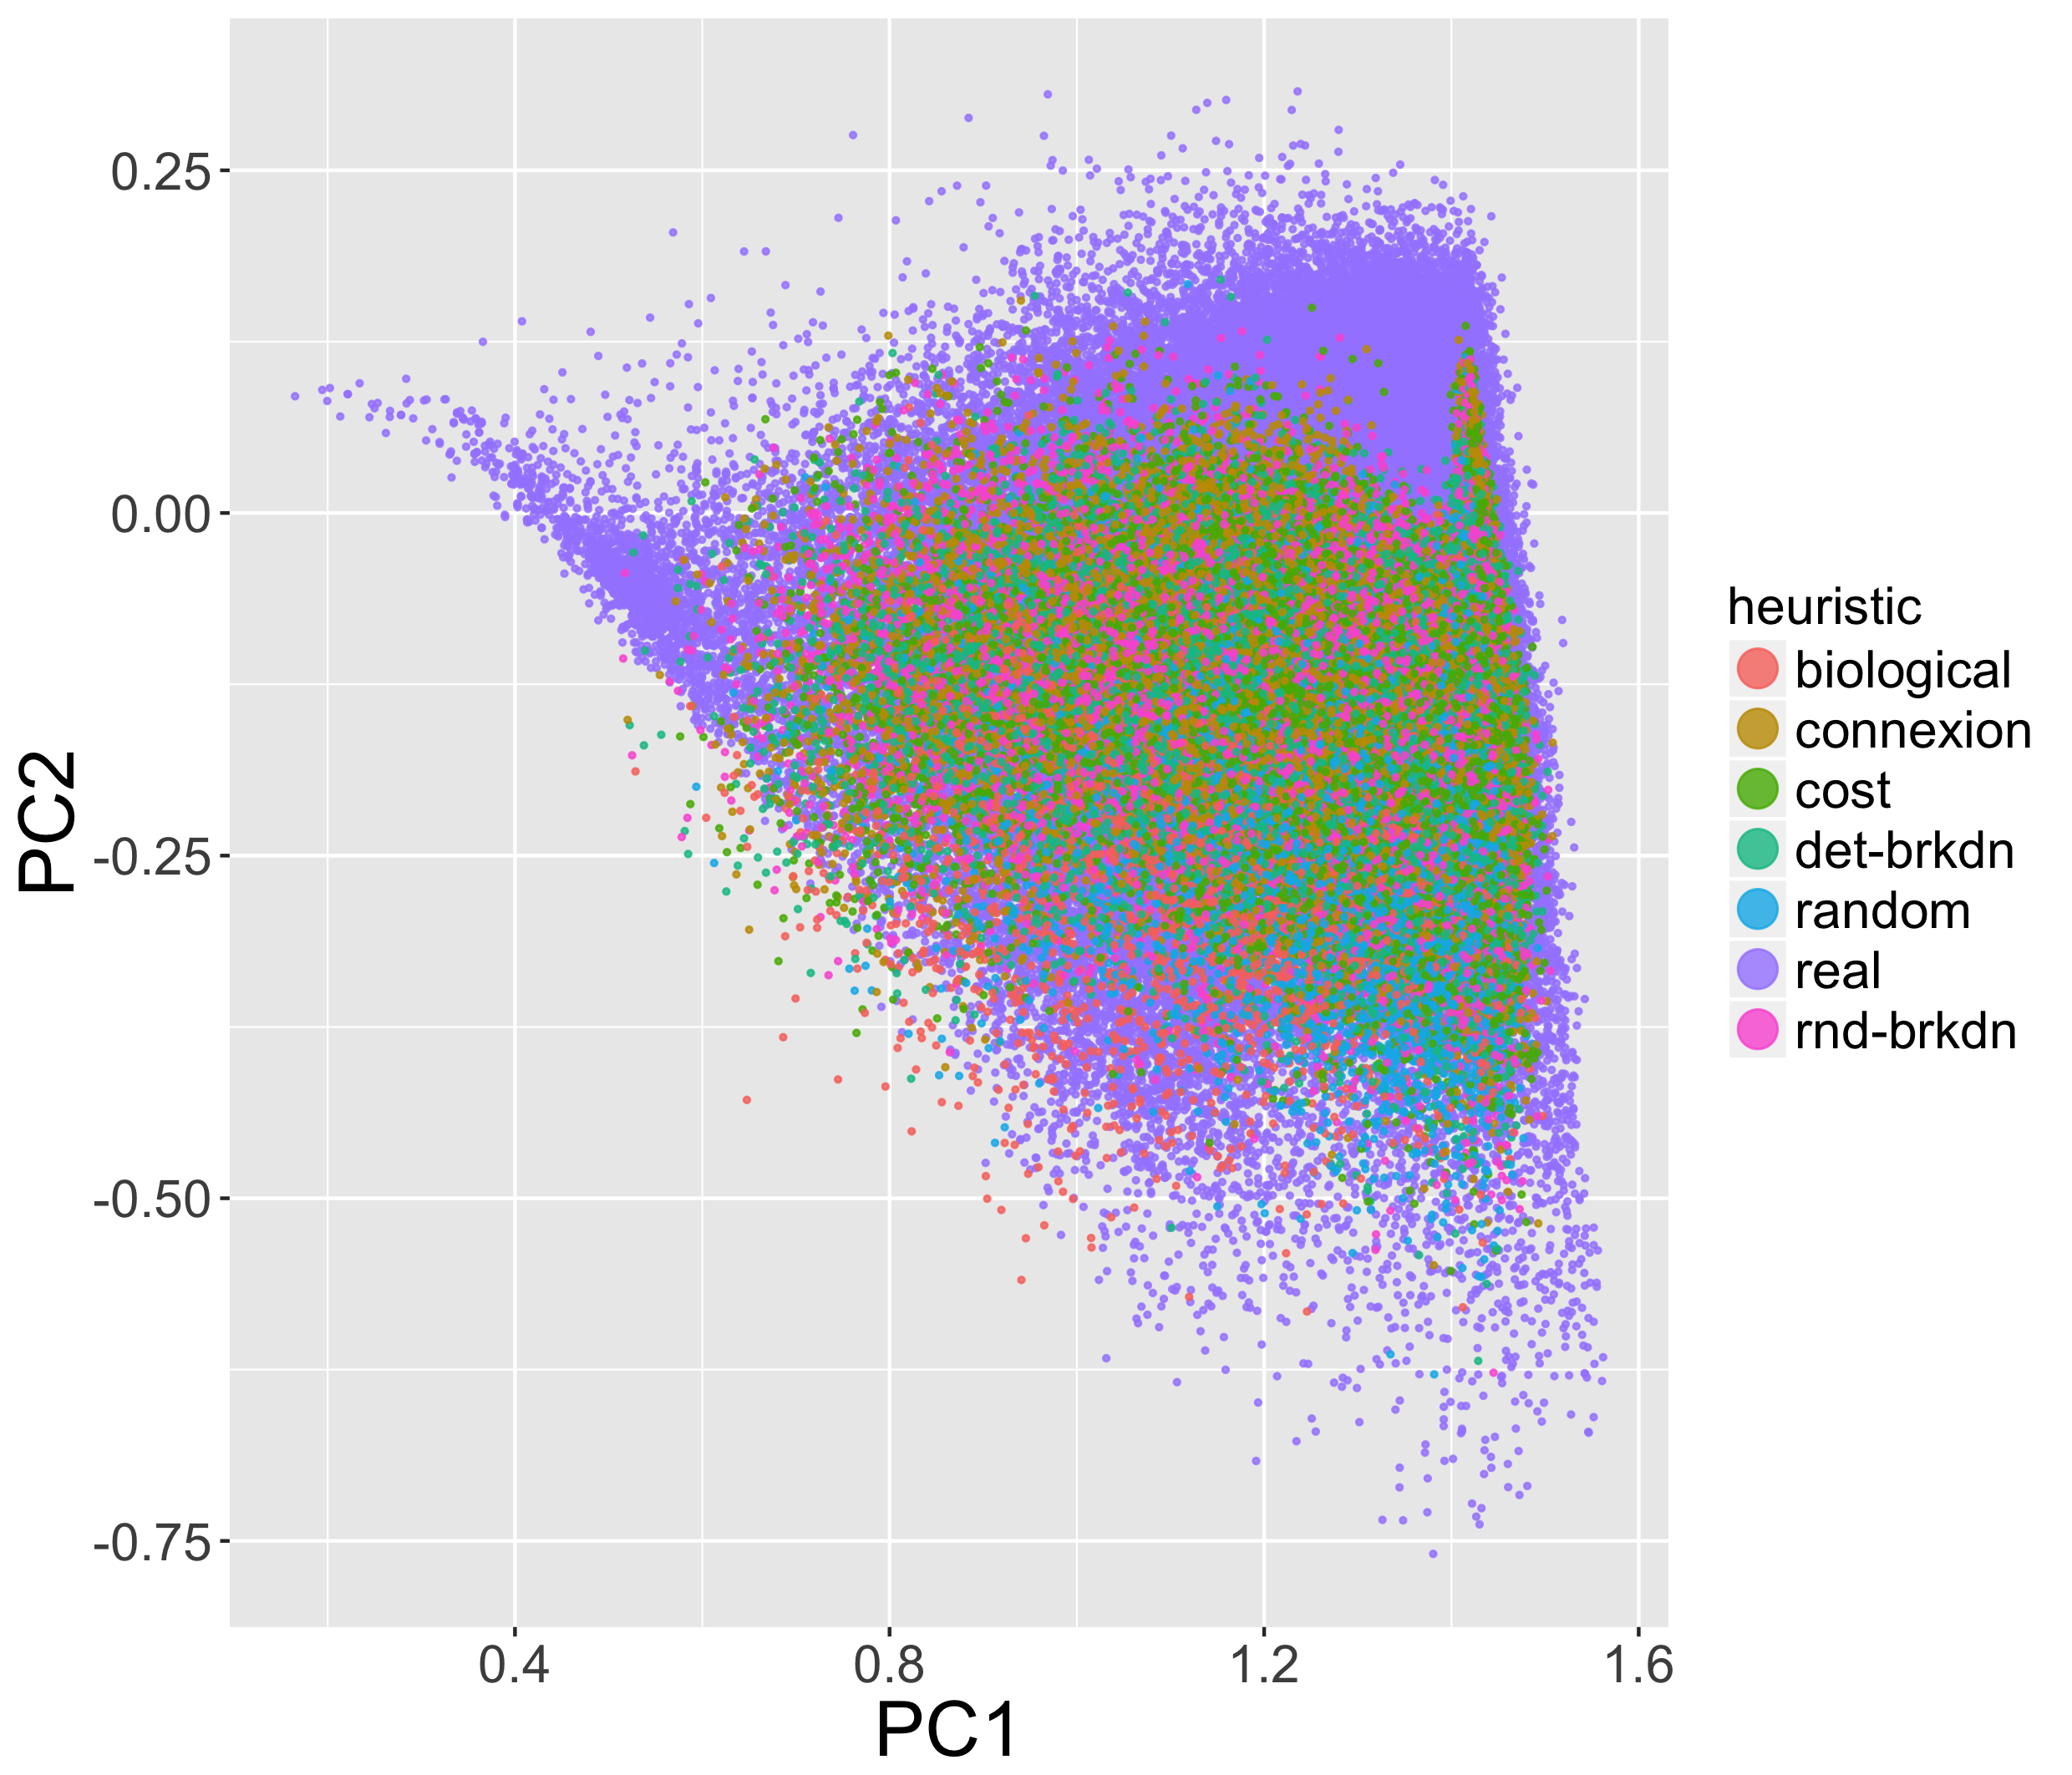
\includegraphics[width=0.48\linewidth]{Figures/MesoCoEvol/pca_morpho_byheuristic}
	%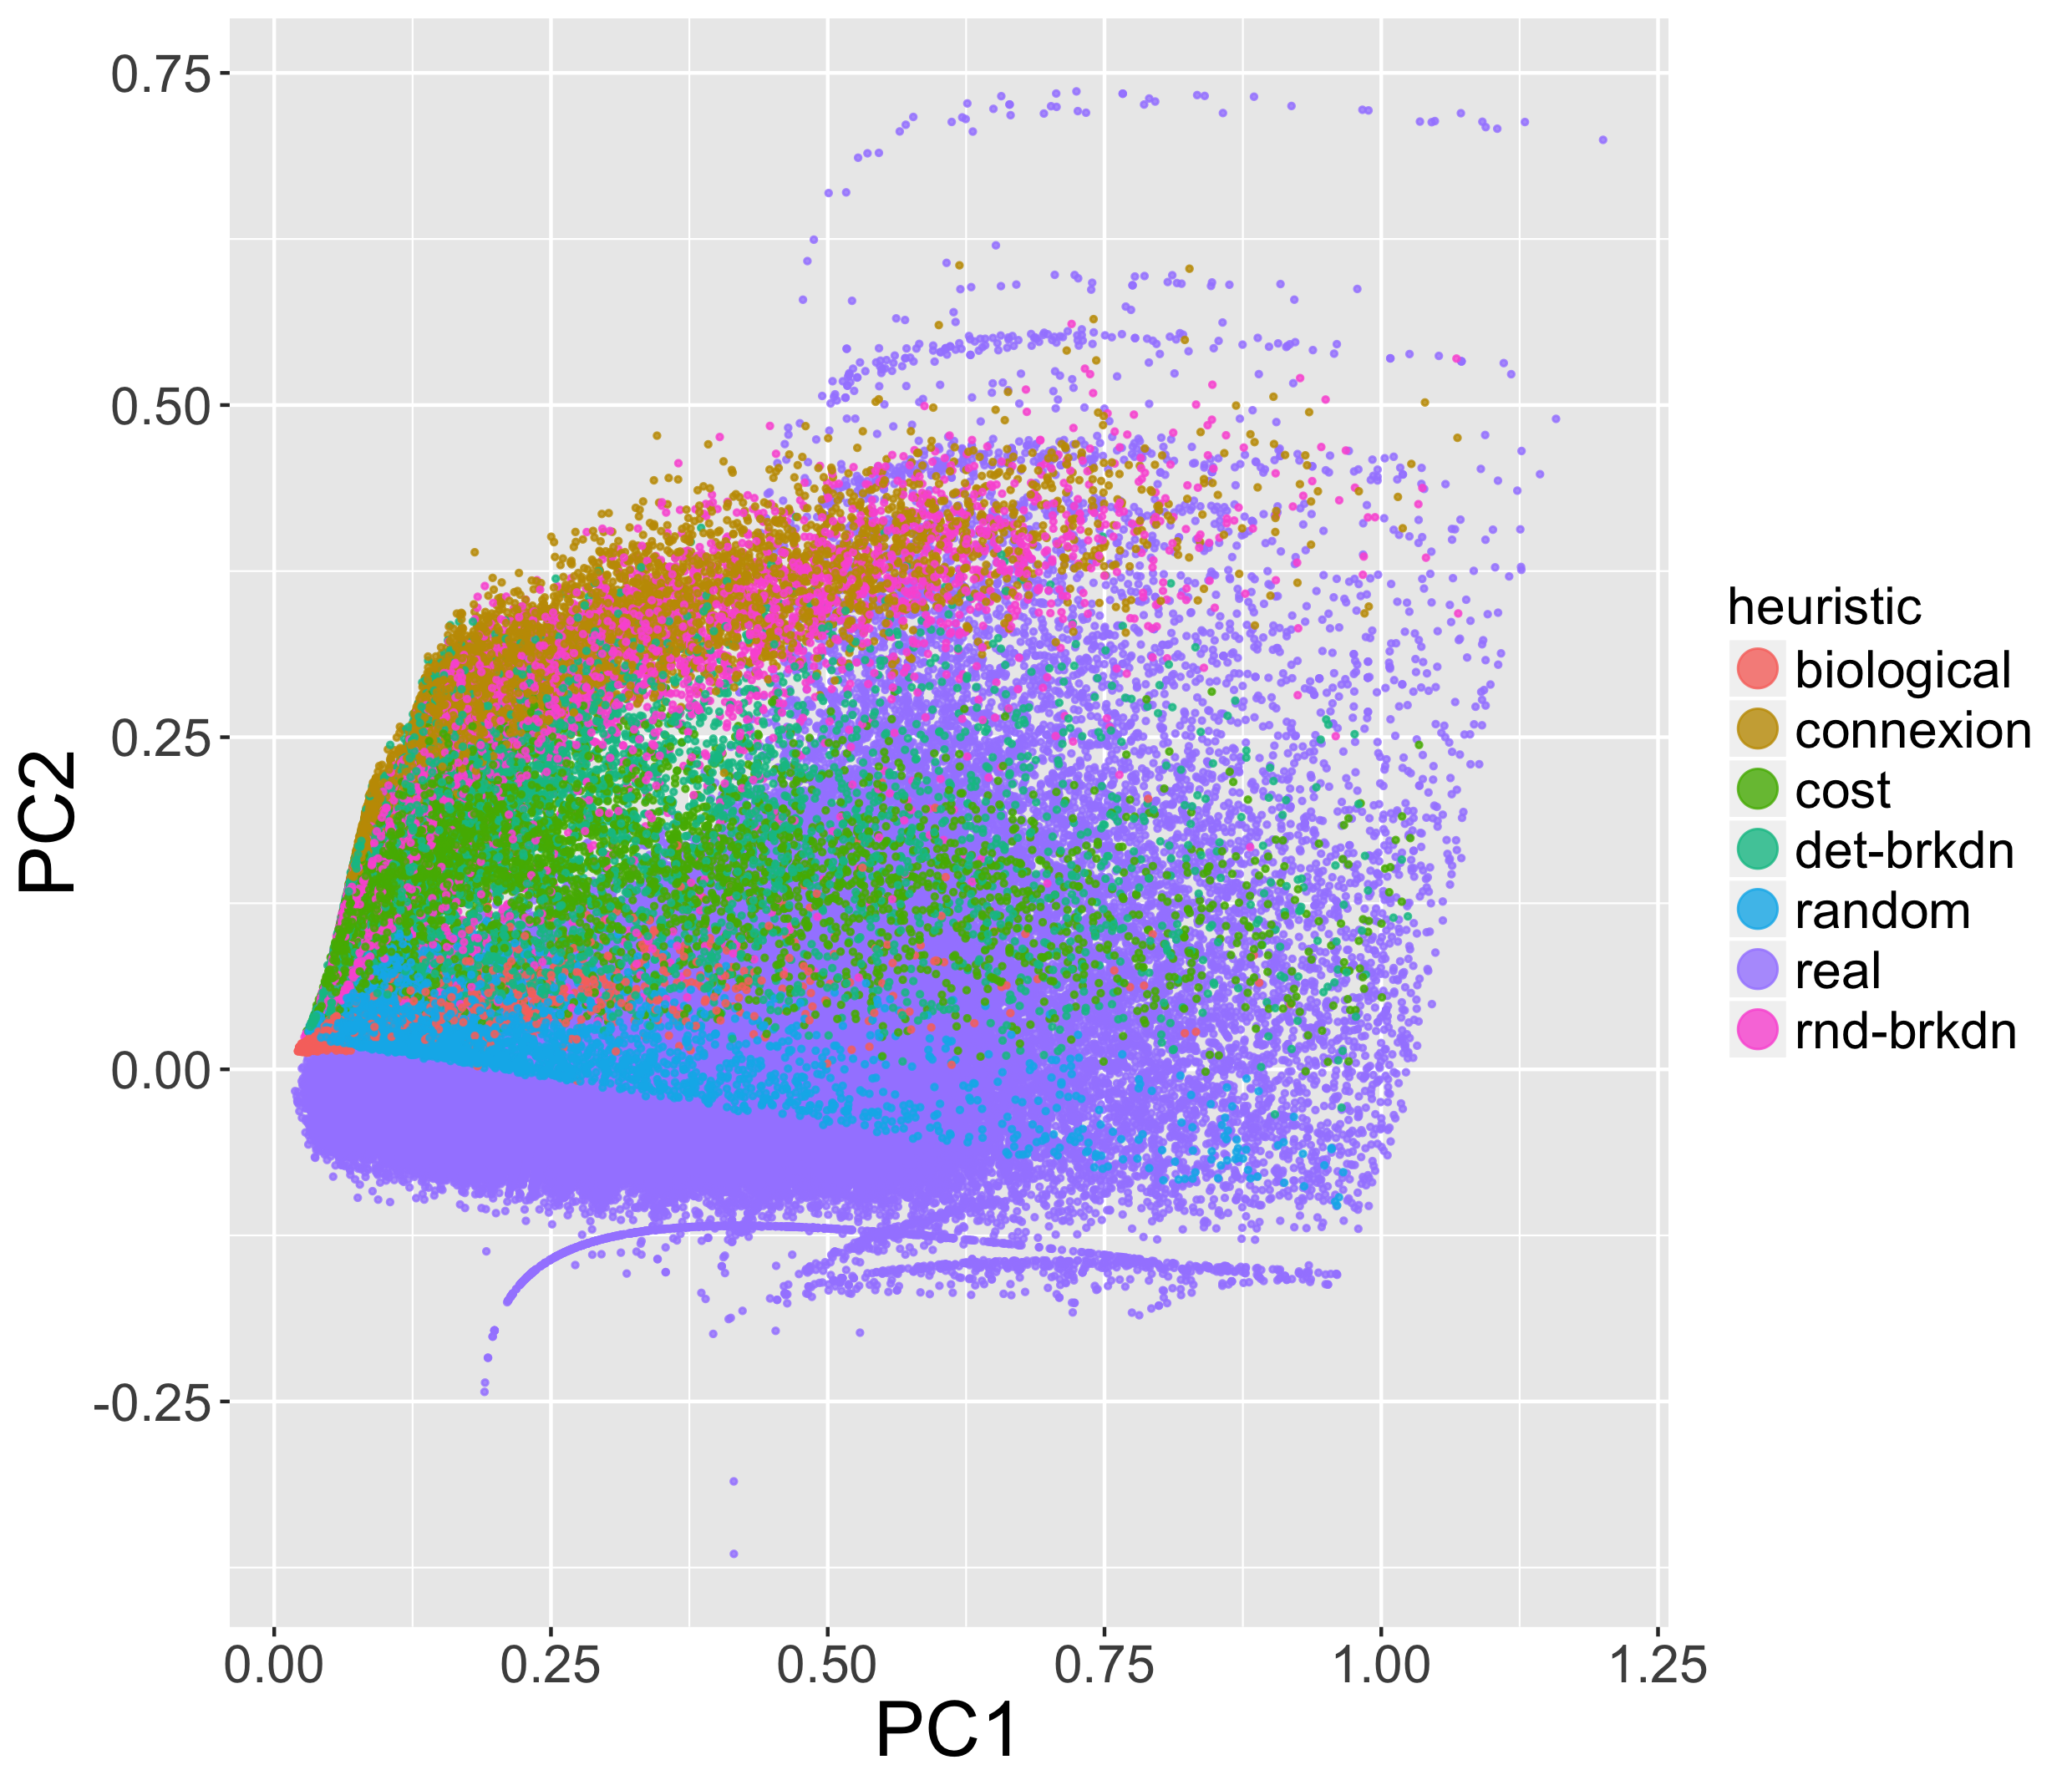
\includegraphics[width=0.48\linewidth]{Figures/MesoCoEvol/pca_network_byheuristic}
	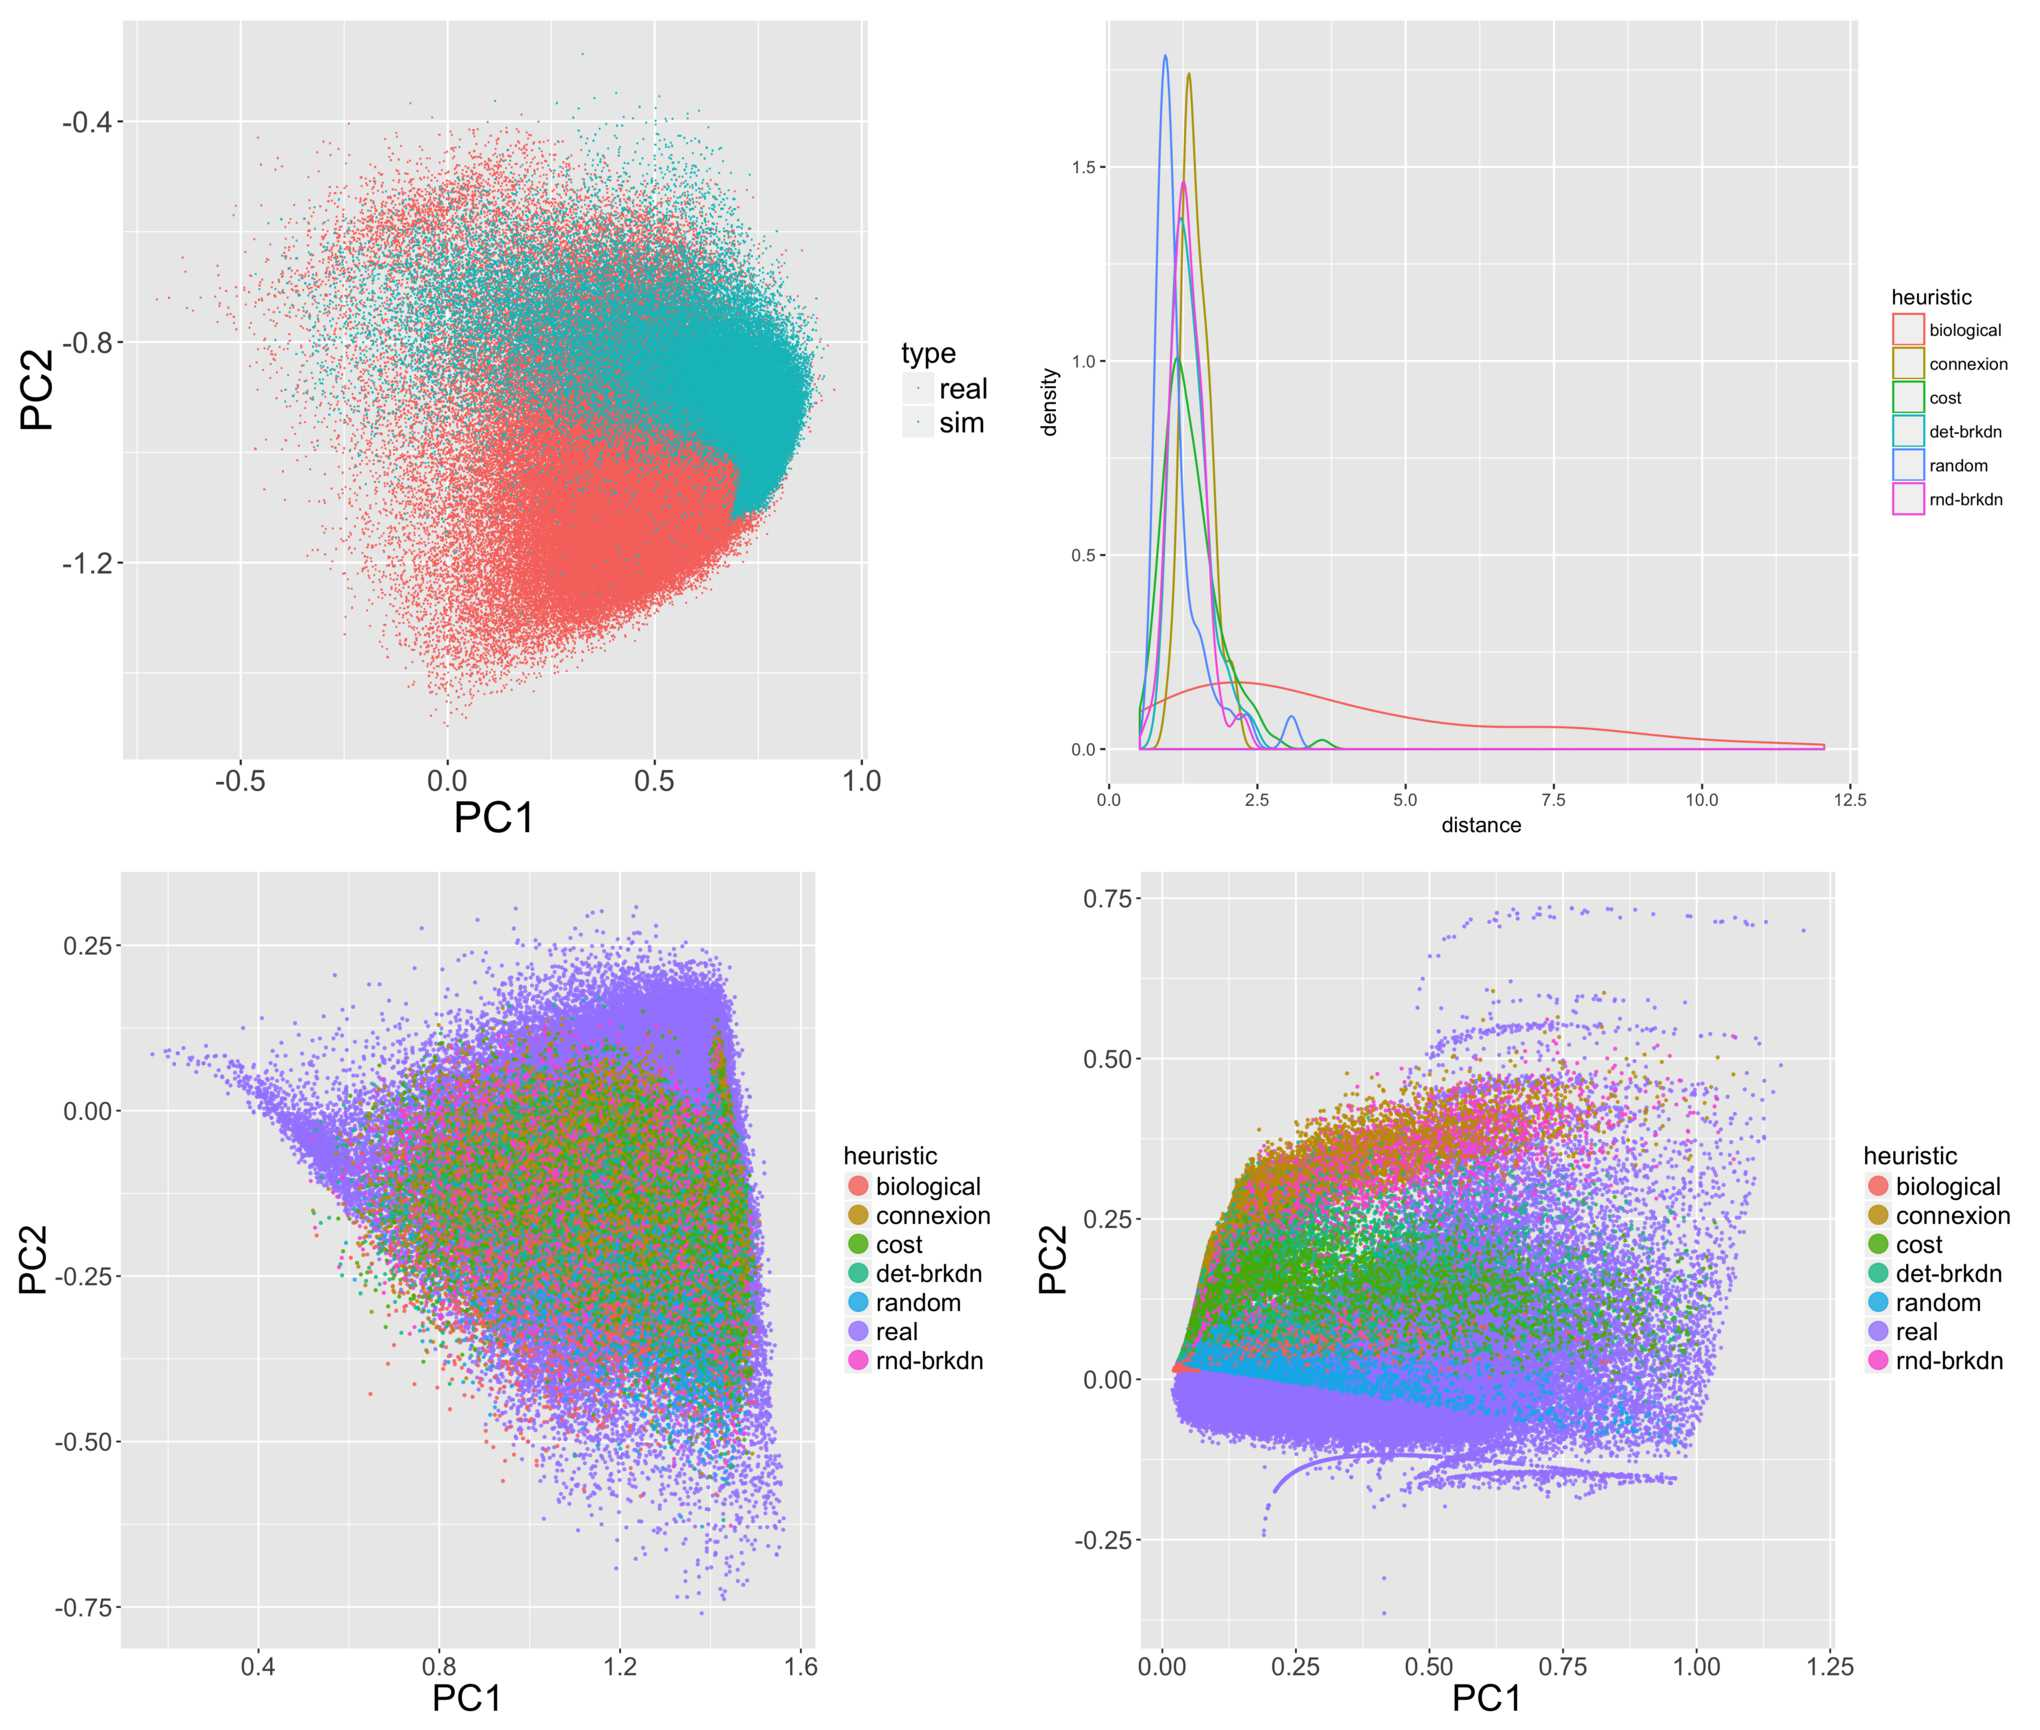
\includegraphics[width=\linewidth]{Figures/Final/7-2-2-fig-mesocoevolmodel-calibration.jpg}
	\caption[Calibration of the morphogenesis model][Calibration du modèle de morphogenèse]{\textbf{Calibration of the morphogenesis model at the first and second order.} (\textit{Top Left}) Simulated and observed point clouds in a principal plan for urban morphology indicators. (\textit{Top Right}) Simulated and observed could points in a principal plan for network indicators. (\textit{Bottom Left}) Simulated and observed point clouds in a principal plan for all indicators. (\textit{Bottom Right}) Distributions of distances on correlations $d_{\rho}$, for the different heuristics.\label{fig:mesocoevolmodel:calibration}}{\textbf{Calibration du modèle de morphogenèse au premier et au second ordre.} (\textit{Haut Gauche}) Nuages de points simulés et observés dans un plan principal pour les indicateurs de forme urbaine. (\textit{Haut Droite}) Nuages de points simulés et observés dans un plan principal pour les indicateurs de réseau. (\textit{Bas Gauche}) Nuages de points simulés et observés dans un plan principal pour l'ensemble des indicateurs. (\textit{Bas Droite}) Distributions des distances sur les corrélations $d_{\rho}$, pour les différentes heuristiques.\label{fig:mesocoevolmodel:calibration}}
\end{figure}
%%%%%%%%%%%%%%%


\bpar{
The model is calibrated at the first order, on indicators for the urban form and network measures, and at the second order on correlations between these. Real data used are still the same as introduced in~\ref{sec:staticcorrelations}, which as we recall it are based on Eurostat population grid and the road network from OpenStreetMap. We use here the full set of points from Europe.
}{
Le modèle est calibré au premier ordre, sur les indicateurs de forme urbaine et de mesure de réseau, ainsi qu'au second ordre sur les correlations entre ceux-ci. Les données réelles utilisées sont toujours celles introduites en~\ref{sec:staticcorrelations}, qui nous le rappelons sont basées sur les données de population raster Eurostat et le réseau routier issu d'OpenStreetMap. Nous utilisons ici l'ensemble des points de l'Europe.
}

\bpar{
We introduce an \emph{ad hoc} calibration procedure in order to take into account the first two moments, that we detail below. More elaborated procedures are used for example in economics, such as \cite{watson1993measures} which uses the noise of the difference between two variables to obtain the same covariance structure for the two corresponding models, or in finance, such as \cite{frey2001copulas} which define a notion on equivalence between latent variables models which incorporates the equality of the interdependence structure between variables. We avoid here to add supplementary models, and consider simply a distance on correlation matrices. The procedure is the following.
\begin{itemize}
	\item Simulated points are the ones obtained through the sampling, with average values on repetitions.
	\item In order to be able to estimate correlation matrices between indicators for simulated data, we make the assumption that second moments are continuous as a function of model parameters, and split for each heuristic the parameter space into areas to group parameter points\footnote{Each parameter being binned into $15 / k$ equal segments, where $k$ is the number of parameters: we empirically observed that this allowed to always have a minimal number of points in each area.}, what allows to estimate for each group indicators and the correlation matrix.
	\item For each estimation done this way, that we write $\bar{S}$ (indicators) and $\rho [S]$ (correlations), we can then compute the distance to real points on indicators $d_I (R_j) = d(\bar{S},R_j)$ and on correlation matrices $d_{\rho} (R_j) = d(\rho [S],\rho[R_j])$ where $R_j$ are the real points with their corresponding correlations\footnote{That are estimated in~\ref{sec:staticcorrelations} as we recall, with a square window centered around the point, that we take here for $\delta = 4$.}, and $d$ an euclidian distance normalized by the number of components.
	\item We consider then the aggregated distance defined as $d_A^2 (R_j) = d_I^2 (R_j) + d_{\rho}^2 (R_j)$. Indeed, as developed empirically and analytically in Appendix~\ref{app:sec:mesocoevolmodel}, the shape of Pareto fronts for the two distances considered suggests the relevance of this aggregation. The real point closest to a simulated point is then the one in the sense of this distance.
\end{itemize}
}{
Nous introduisons un processus \emph{ad hoc} de calibration pour pouvoir tenir compte des deux premiers moments, que nous détaillons ci-dessous. Des procédures plus élaborées sont utilisées par exemple en économie, comme \cite{watson1993measures} qui utilise le bruit de la différence entre deux variables pour obtenir la même structure de covariance pour les deux modèles correspondants, ou en finance, comme \cite{frey2001copulas} qui définissent une notion d'équivalence entre modèles à variables latentes qui incorpore l'égalité de la structure d'interdépendance entre variables. Nous évitons ici d'ajouter des modèles supplémentaires, et considérons simplement une distance sur les matrices de corrélation. La procédure est la suivante.
\begin{itemize}
	\item Les points simulés sont ceux issus de l'échantillonnage, avec les valeurs moyennes sur les répétitions.
	\item Afin de pouvoir estimer des matrices de corrélation entre indicateurs pour les données simulées, nous faisons l'hypothèse que les seconds moments sont continus en les paramètres du modèle, et découpons pour chaque heuristique l'espace des paramètres en zones pour grouper les points de paramètres\footnote{Chaque paramètre étant découpé en $15 / k$ segments égaux avec $k$ nombre de paramètres : nous avons constaté empiriquement que cela permettait d'avoir toujours un nombre minimal de mesures dans chaque zone.}, ce qui permet d'estimer pour chaque groupe les indicateurs et la matrice des corrélations.
	\item Pour chaque estimation ainsi menée, qu'on note $\bar{S}$ (indicateurs) et $\rho [S]$ (corrélations), on peut alors calculer la distance aux points réels sur les indicateurs $d_I (R_j) = d(\bar{S},R_j)$ et sur les matrices de corrélation $d_{\rho} (R_j) = d(\rho [S],\rho[R_j])$ où les $R_j$ sont les points réels avec leurs corrélations correspondantes\footnote{Estimées on le rappelle en~\ref{sec:staticcorrelations}, par fenêtre centrée sur le point, qu'on prend ici pour $\delta = 4$.}, et $d$ une distance euclidienne normalisée par le nombre de composantes.
	\item Nous considérons alors la distance agrégée définie comme $d_A^2 (R_j) = d_I^2 (R_j) + d_{\rho}^2 (R_j)$. En effet, comme développé empiriquement et analytiquement en Annexe~\ref{app:sec:mesocoevolmodel}, la forme des fronts de Pareto pour les deux distances considérées suggère la pertinence de cette agrégation. Le point réel le plus proche du point simulé est alors celui au sens de cette distance.
\end{itemize}
}






\bpar{
The Fig.~\ref{fig:mesocoevolmodel:calibration} summarizes calibration results. Morphological indicators are easier to approach than network indicators, for which a part of the simulated clouds does not superpose with observed points. We find again a certain complementarity between network heuristics. When considering the full set of indicators, few simulated points are situated far from the observed points, but a significant proportion of these is beyond the reach of simulation. Thus, the simultaneous capture of morphology and topology is obtained at the price of less precision.
}{
La Fig.~\ref{fig:mesocoevolmodel:calibration} résume les résultats de la calibration. Les indicateurs morphologiques sont plus aisément approchés que ceux de réseau, pour lesquels une partie des nuages simulés ne se superpose pas avec les points observés. Nous retrouvons une certaine complémentarité dans les heuristiques de réseau. En considérant l'ensemble des indicateurs, peu de points simulés tombent loin des points observés, mais une proportion significative de ceux-ci est hors d'atteinte de la simulation. Ainsi, la capture simultanée de la morphologie et de la topologie se fait au prix d'une moins grande précision.
}

\bpar{
We however obtain a good reproduction of correlation matrices as shown in Fig.~\ref{fig:mesocoevolmodel:calibration} (histogram for $d_{\rho}$, bottom right). The worse heuristic for correlations is the biological one in terms of maximum, whereas the random produces rather good results: this could be due for example to the reproduction of very low correlations, which accompany a structure effect due to the initial addition of nodes which imposes already a certain correlation. On the contrary, the biological heuristic introduces supplementary processes which can possibly be beneficial to the network in terms of independence (or following the opposed viewpoint be detrimental in terms of correlations). In any case, this application shows that our model is able to resemble real configurations both for indicators and their correlations.
}{
Nous obtenons toutefois une bonne reproduction des matrices de corrélation, comme présenté en Fig.~\ref{fig:mesocoevolmodel:calibration} (histogramme de $d_{\rho}$, bas droite). La moins bonne heuristique pour les corrélations est la biologique en termes de maximum, tandis que l'aléatoire produit d'assez bons résultats : cela pourrait par exemple être dû à la reproduction des corrélations quasi nulles, accompagnant un effet de structure dû à l'ajout initial des noeuds qui impose déjà une certaine corrélation. Au contraire, l'heuristique biologique introduit des processus supplémentaires qui peuvent éventuellement bénéficier au réseau en termes d'indépendance (ou selon le point de vue opposé être préjudiciable en termes de corrélations). En tout cas, cette application démontre que notre modèle est capable à la fois de s'approcher de configurations réelles pour les indicateurs et pour leurs corrélations.
}






\subsubsection{Causality regimes}{Régimes de causalité}



\bpar{
We furthermore study dynamical lagged correlations between the variations of the different explicative variables for cells (population, distance to the network, closeness centrality, betweenness centrality, accessibility). We apply the method of causality regimes introduced in~\ref{sec:causalityregimes}. The Fig.~\ref{fig:mesocoevolmodel:causality} summarizes the results obtained with the application of this method on simulation results of the co-evolution model. The number of classes inducing a transition is smaller than for the RDB model, translating a smaller degree of freedom, and we fix in that case $k=4$. Centroid profiles allow to understand to ability of the model to more or less capture a co-evolution.
}{
Nous étudions d'autre part les correlations retardées dynamiques entre les variations des différentes variables explicatives des cellules (population, distance au réseau, centralité de proximité, centralité de chemin, accessibilité). Nous appliquons la méthode des régimes de causalité introduite en~\ref{sec:causalityregimes}. La Fig.~\ref{fig:mesocoevolmodel:causality} résume les résultats obtenus par l'application de cette méthode sur les résultats de simulation du modèle de co-évolution. Le nombre de classes induisant une transition est plus faible que pour le modèle RDB, traduisant un plus faible degré de liberté, et nous fixons dans ce cas $k=4$. Les profils des centroïdes permettent de comprendre la capacité du modèle à capturer plus ou moins une co-évolution.
}


% reg 1 : network suit pop ; reg 2 : idem mais pas dans strucutre locale (pop road $\simeq 0$) ; reg3 : nw suit mais que local, pas structure. ; reg 4 : bw anticause access : network and pop avoid congestion ; plus nw suit : somehow circulaire, vraie co-evol ?


\bpar{
The regimes obtained appear to be less diverse than the ones obtained in~\ref{sec:causalityregimes} or for the macroscopic co-evolution in~\ref{sec:macrocoevol}. Some variables have naturally a strong simultaneous correlation, spurious from their definitions, such as closeness centrality and accessibility, or the distance to the road and the closeness centrality. For all regimes, population significantly determines the accessibility. The regime 1 corresponds to a full determination of the network by the population. The second is partly circular, through the effect of roads on populations. The regime 3 is more interesting, since closeness centrality negatively causes the accessibility: this means that in this configuration, the coupled evolution of the network and the population follow the direction of a diminution of congestion. Furthermore, as population causes the closeness centrality, there is also circularity and thus co-evolution in that case. When we locate it in the phase diagram, this regime is rather sparse and rare, contrary for example to the regime 1 which occupies a large portion of space for a low importance of the road ($w_{road} \leq 0.3$). This confirms that the co-evolution produced by the model is localized and not a characteristic always verified, but that it is however able to generate some in particular regimes.
}{
Les régimes obtenus apparaissent moins divers que ceux obtenus en~\ref{sec:causalityregimes} ou pour la co-évolution macroscopique en~\ref{sec:macrocoevol}. Certaines variables ont naturellement une forte corrélation simultanée, fortuite par leur définitions, comme la centralité de proximité et l'accessibilité, ou la distance à la route et la centralité de proximité. Dans l'ensemble des régimes, la population détermine significativement l'accessibilité. Le régime 1 correspond à une détermination entière du réseau par la population. Le second est partiellement circulaire, de par l'effet des routes sur la population. Le régime 3 est intéressant, la centralité de chemin causant négativement l'accessibilité : cela veut dire que dans cette configuration, l'évolution couplée du réseau et de la population vont dans le sens d'une diminution de la congestion. De plus, comme la population cause la centralité de proximité, il y a également circularité et donc co-évolution dans ce cas. En le localisant dans le diagramme de phase, ce régime est assez dispersé et rare, au contraire par exemple du régime 1 qui occupe une grande partie de l'espace pour une importance faible de la route ($w_{road} \leq 0.3$). Cela confirme que la co-évolution produite par le modèle est ponctuelle et non une caractéristique toujours vérifiée, mais qu'il est toutefois capable d'en générer dans des régimes particuliers.
}


%%%%%%%%%%%%%%%
\begin{figure}
	%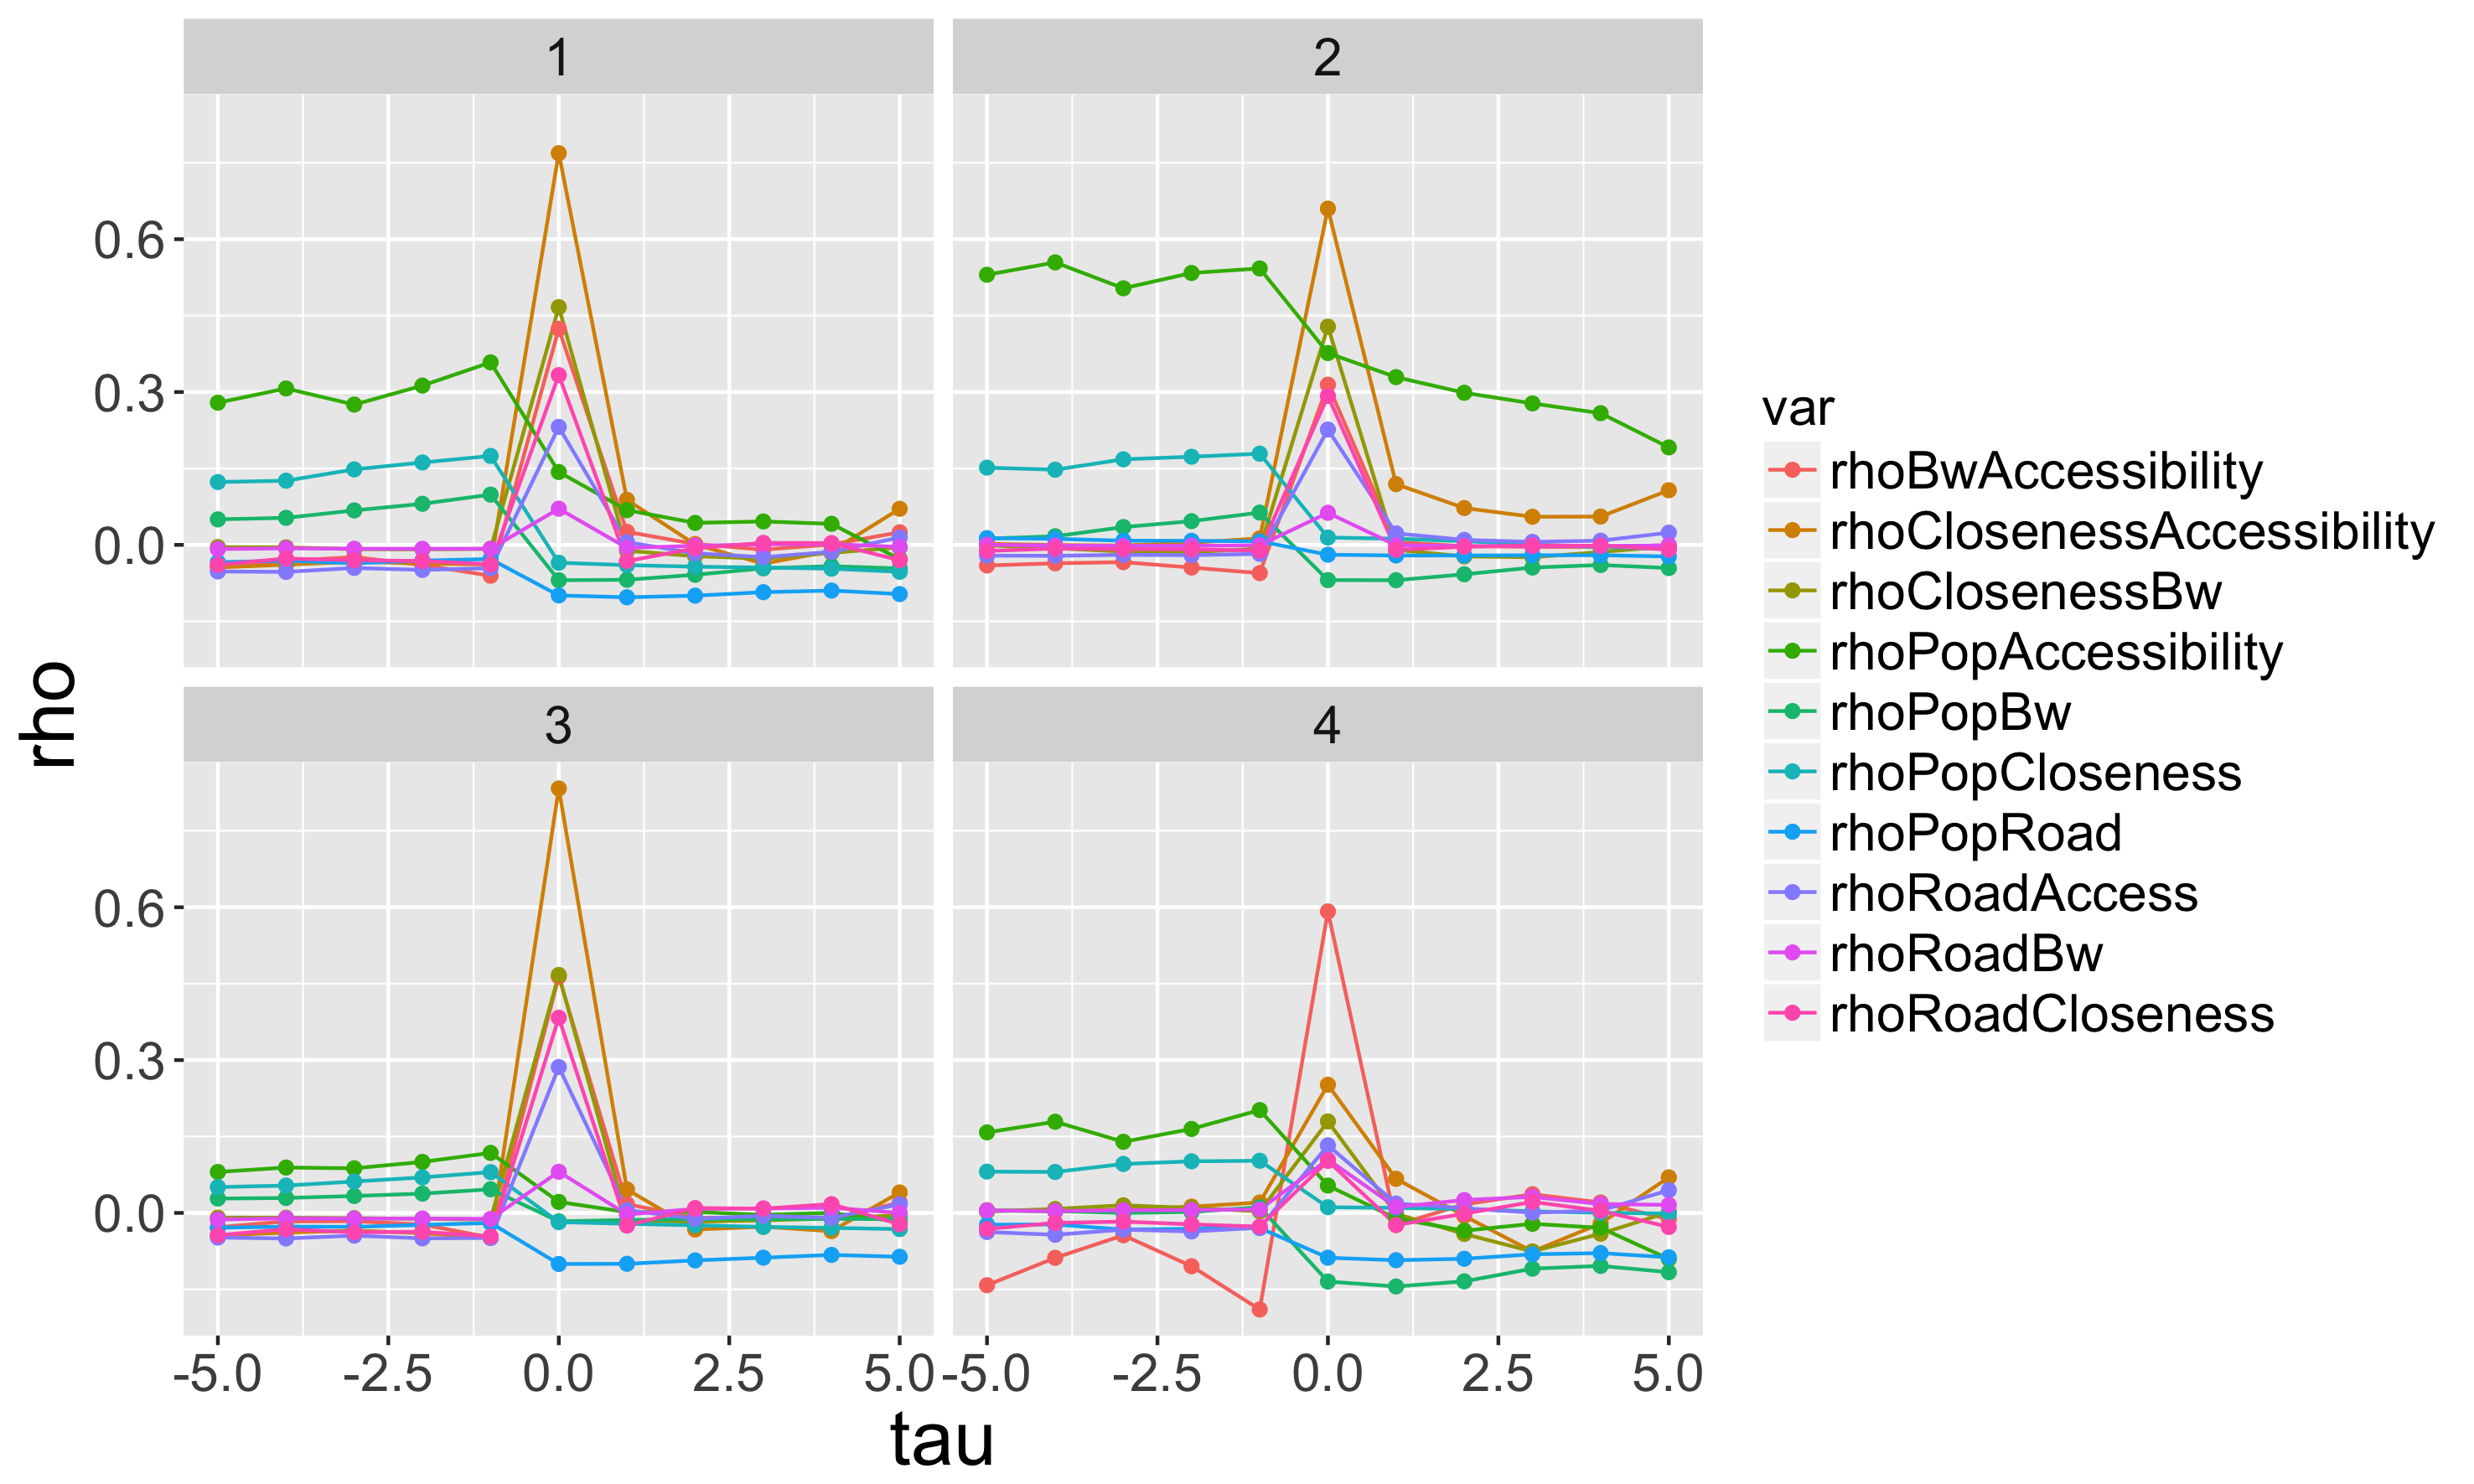
\includegraphics[width=0.53\linewidth]{Figures/MesoCoEvol/centertrajs}
	%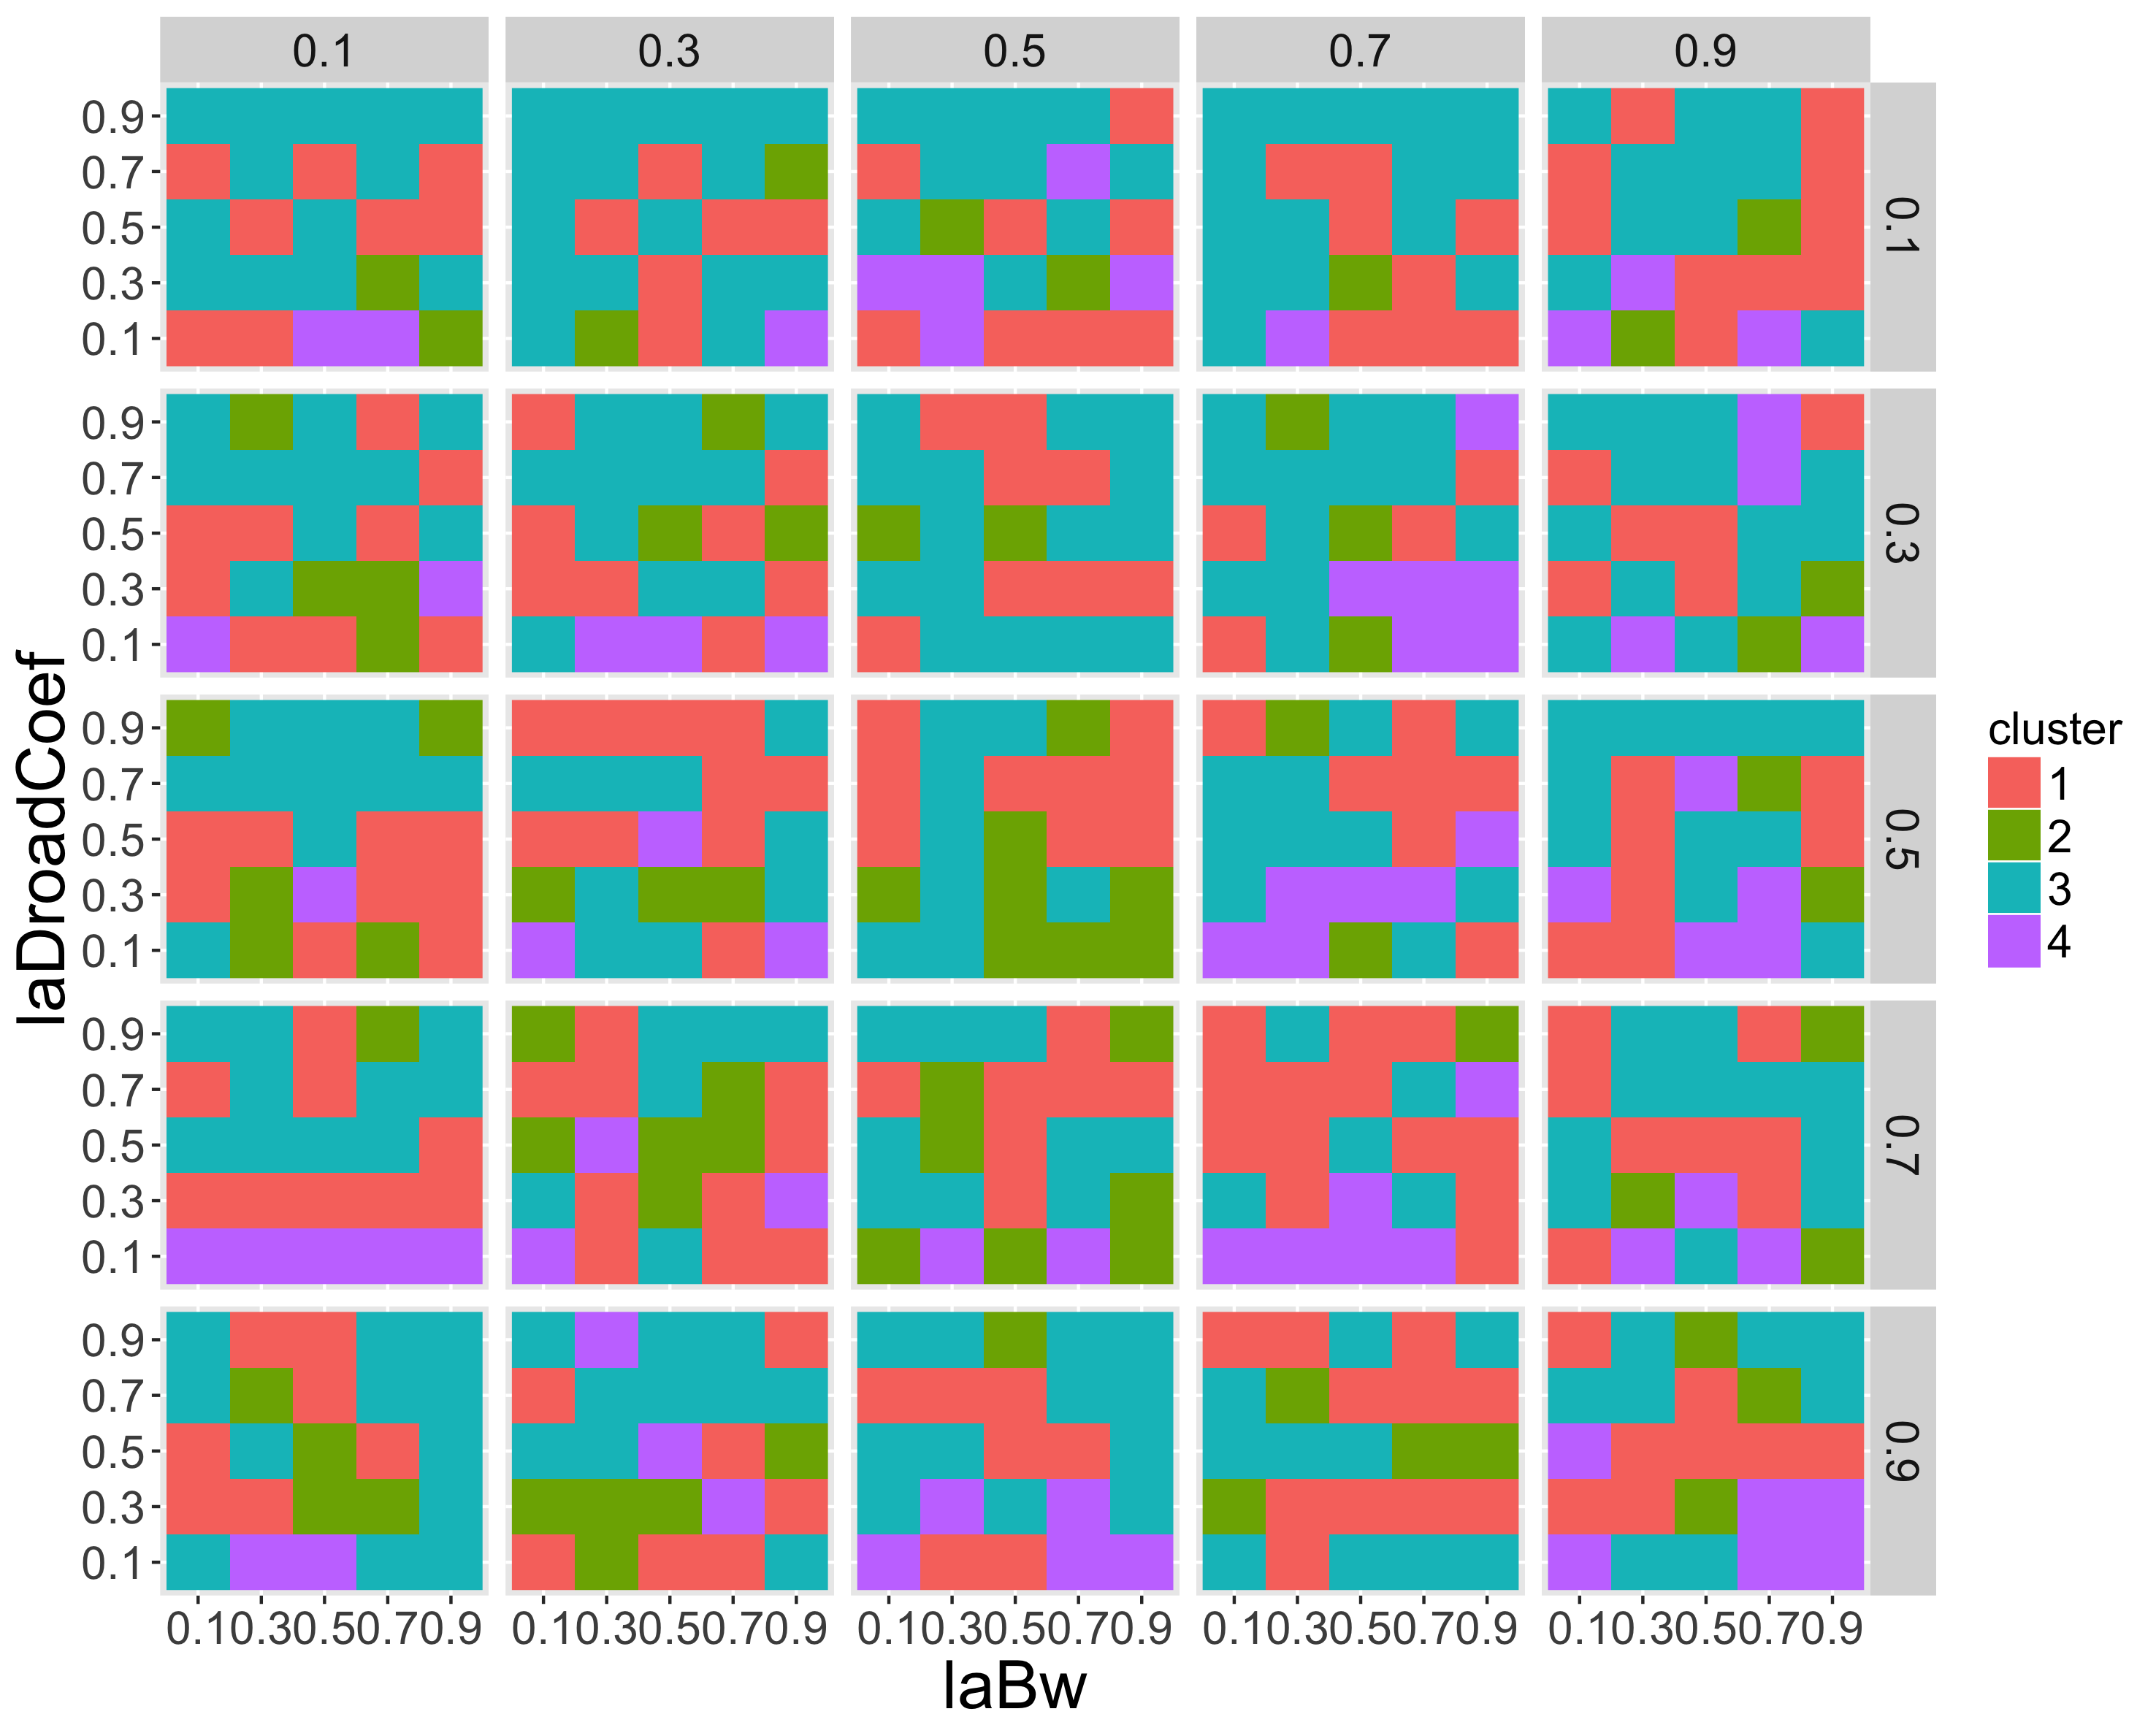
\includegraphics[width=0.44\linewidth]{Figures/MesoCoEvol/cluster-params}
	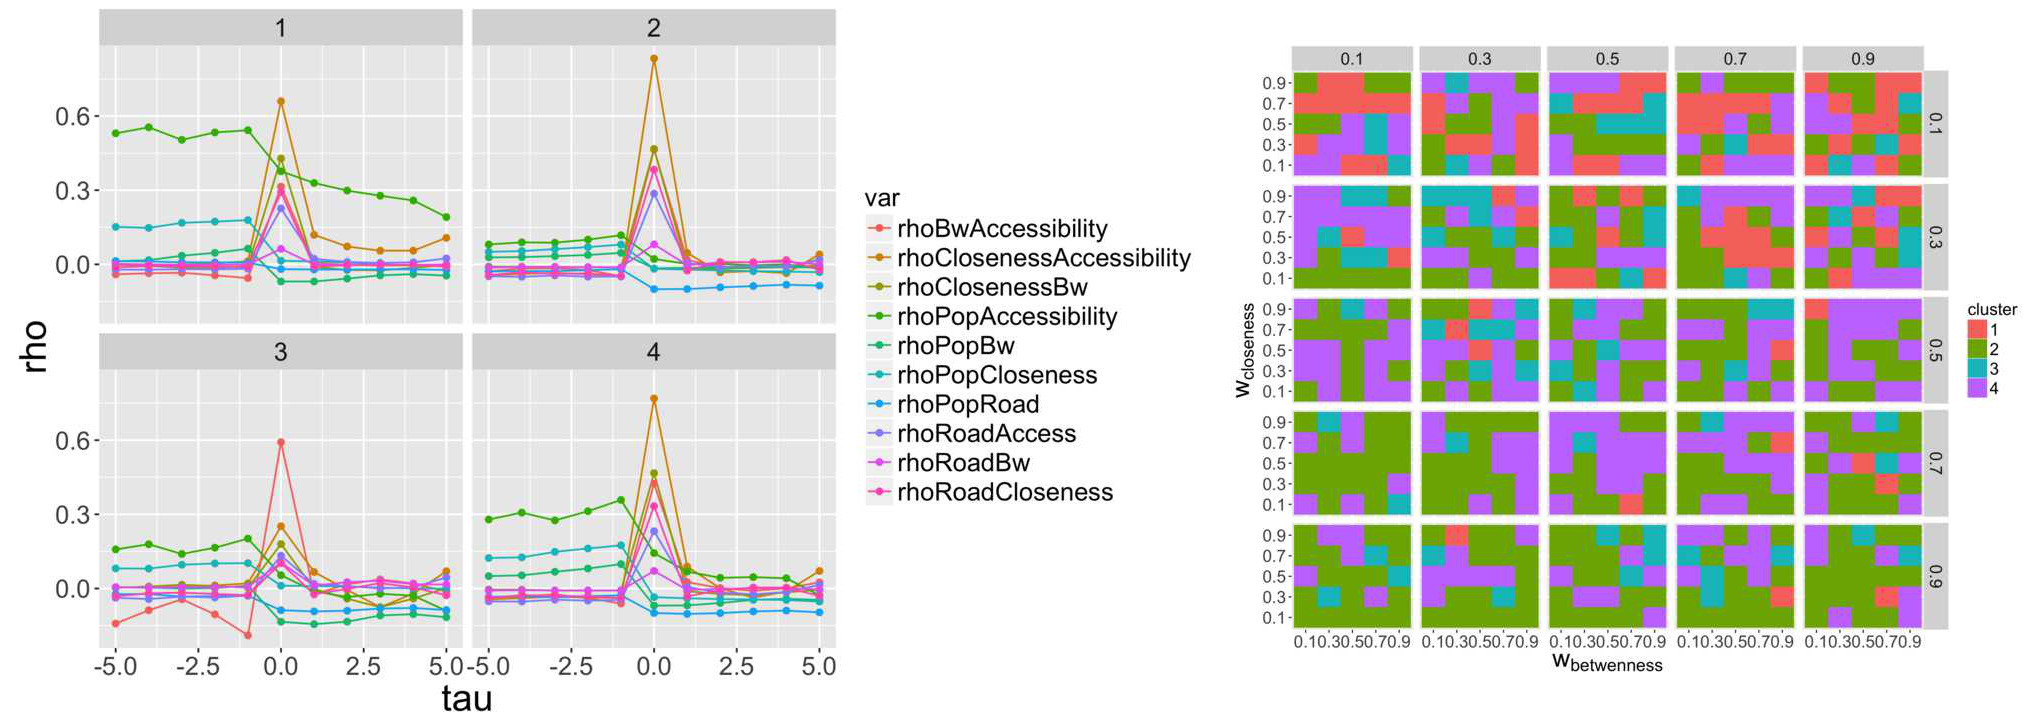
\includegraphics[width=\linewidth,height=0.93\textheight]{Figures/Final/7-2-2-fig-mesocoevolmodel-causality}
	\caption[Causality regimes for the morphogenesis model][Régimes de causalité pour le modèle de morphogenèse]{\textbf{Causality regimes for the co-evolution model.} (\textit{Top}) Trajectories of classes centers in terms of $\rho[\tau]$ between the different explicative variables. (\textit{Bottom}) Phase diagram of regimes in the parameter space for $w_k$, represented here as the variation of diagrams for $(w_{bw},w_{cl})$, along the variations of $w_{road}$ (in rows) and of $w_{pop}$ (in columns).\label{fig:mesocoevolmodel:causality}}{\textbf{Régimes de causalité pour le modèle de co-évolution.} (\textit{Haut}) Trajectoire des centres des classes en termes de $\rho[\tau]$ entre les différentes variables explicatives. (\textit{Bas}) Diagramme de phase des régimes dans l'espace des paramètres $w_k$, représenté ici comme la variation des diagrammes pour $(w_{bw},w_{cl})$, selon les variations de $w_{road}$ (en ligne) et de $w_{pop}$ (en colonne). \label{fig:mesocoevolmodel:causality}}
\end{figure}
%%%%%%%%%%%%%%%





%%%%%%%%%%%%%%%
\subsection{Discussion}{Discussion}

%\comment[JR]{\cite{blumenfeld2010network} : hybrid model (largely discussed by Clara) ; network growth induces migration ; would be interesting to test its abilities to produce various causality regimes (note : may be one indicator of how a model captures co-evolution ?)}


\bpar{
We have thus proposed a co-evolution model at the mesoscopic scale, based on a multi-modeling paradigm for the evolution of the network. The model is able to reproduce a certain number of observed situations at the first and second order, capturing thus a static representation of interactions between networks and territories. It also yields different dynamical causality regimes, being however less diverse than the simple model studied before: therefore, a more elaborated structure in terms of processes must be paid in flexibility of interaction between these. This suggests a tension between a ``static performance'' and a ``dynamical performance'' of models.
}{
Nous avons ainsi proposé un modèle de co-évolution à l'échelle mesoscopique, se basant sur un paradigme de multi-modélisation pour l'évolution du réseau. Le modèle est capable de reproduire un certain nombre de situations observées au premier et au second ordre, capturant une représentation statique des interactions entre réseaux et territoires. Il dégage également différents régimes dynamiques de causalité, en étant toutefois moins riche que le modèle simple étudié plus tôt : ainsi, une structure plus élaborée en termes de processus se paie en flexibilité d'interaction entre ceux-ci. Cela suggère une tension entre ``performance statique'' et ``performance dynamique'' des modèles.
}


%%%%%%
% Rq : ces conclusions sont legeres sans un PSE ou un reverse image..
%  -> big developements pour plus tard !
%  : ex calib par region geographique.
% idem perf statique / dynamique : a creuser pour les histoires de validation de modeles ?
%
% -> le modele reseau pur comme baseline : back to representation of territorial systems !

\bpar{
An open question is to what extent a pure network model with preferential attachment for nodes would reproduce results close to what we obtained. The complex coupling between aggregation and diffusion (shown in~\ref{sec:densitygeneration}) could not be easily included, and the model could in any case not answer to questions on the coupling of the dynamics.
}{
Une question ouverte est dans quelle mesure un modèle de réseau pur avec attachement préférentiel des noeuds reproduirait des résultats proches des nôtres. Le couplage complexe entre agrégation et diffusion (montré en~\ref{sec:densitygeneration}) ne pourrait pas être inclut aisément, et le modèle ne pourrait dans tous les cas répondre à des problématiques concernant le couplage des dynamiques.
}


%Cette réflexion rejoint la question des représentations territoriales que nous aborderons en ouverture.
%\comment[JR]{develop on Elsa's comment, why just the network with prefatt ? more subtle and want to reproduce coupled dynamics. could suit at the first order ? surely as density-only model performs quite well on morphology only. question of territorial representations, what is necessary, what is an objective, what is both. dimension of urban system.}


\stars


\bpar{
We have thus explored a co-evolution model based on morphogenesis that takes into account multiple processes for the evolution of the network. We studied its calibration on observed data at the first and the second order, and explored the causality regimes it produces.
}{
Nous avons ainsi exploré un modèle de co-évolution se reposant sur la morphogenèse et prenant en compte de multiples processus d'évolution du réseau. Nous avons étudié sa calibration sur données observées au premier et second ordre, et exploré les régimes de causalité qu'il produit.
}


\bpar{
We propose now a last entry into co-evolution at the mesoscopic scale, by developing a model that considerably complexifies the influence of the territory on the network, by taking into account governance processes.
}{
Nous proposons à présent une dernière incursion dans la co-évolution à l'échelle mesoscopique, en développant un modèle qui complexifie considérablement l'influence du territoire sur le réseau, en prenant en compte des processus de gouvernance. 
}



\stars






